\documentclass[a4paper,12pt,twoside]{report}

\usepackage{acronym}
\usepackage{url}
\usepackage{cite}
\usepackage{listings}
\usepackage[pdftex]{graphicx}
\usepackage[hang,small,bf]{caption}
\usepackage{styles/tum}
\usepackage{styles/usecases}
\usepackage{setspace}
\usepackage[german,english]{babel}
\usepackage{float}
\usepackage{floatflt}
\usepackage{fancyhdr}
\usepackage{color}
\usepackage{booktabs}
\usepackage[pdftex,bookmarks=true,plainpages=false,pdfpagelabels=true]{hyperref}
\usepackage{mdwlist}
\usepackage{enumerate}
\usepackage{paralist}
\usepackage{array}
\usepackage{longtable}
\usepackage{listings}
\usepackage[utf8]{inputenc}
\usepackage[capitalize, noabbrev]{cleveref}

% Path for graphics
\graphicspath{{figures/}}

\begin{document}
\setlength{\evensidemargin}{22pt}
\setlength{\oddsidemargin}{22pt}

\def\doctype{Master's Thesis}
\def\faculty{Informatik}
\def\title{Using Synthetic Data for Classification of Small Parts}		%TODO add title in German
\def\titleGer{Synthetische Daten für die Klassifizierung von Kleinteilen verwenden}	%TODO add title in German
\def\supervisor{Prof. Bernd Brügge, Ph.D.}
\def\advisor{Sajjad Taheri, M.Sc.}
\def\author{Amr Abdelraouf}
\def\date{15.10.2018}		%TODO add submission / handover date


\hypersetup{pdfborder={0 0 0},
                        pdfauthor={Amr Abdelraouf},
                        pdftitle={Using Synthetic Data for Classification of Small Parts},
                        }

\lstset{showspaces=false, numbers=left, frame=single, basicstyle=\small}

\pagenumbering{alph}

\thispagestyle{empty}

\vspace{4cm}
\begin{center}
\oTUM{4cm}\\ 
\vspace{5mm}     
\huge FAKULT{\"A}T F{\"U}R INFORMATIK\\ 
\vspace{0.5cm}
\large DER TECHNISCHEN UNIVERSIT{\"A}T M{\"U}NCHEN\\
\vspace{1mm}
\end{center}

\vspace{13mm}

\begin{center}
{\Large \doctype\ in \faculty}
\vspace{20mm}

\begin{spacing}{1.5}
{\huge\bf \title}\\%[3ex]
\end{spacing}

\vspace{15mm}
{\LARGE \author}

\vspace{10mm}

\begin{figure}[h!]
\centering
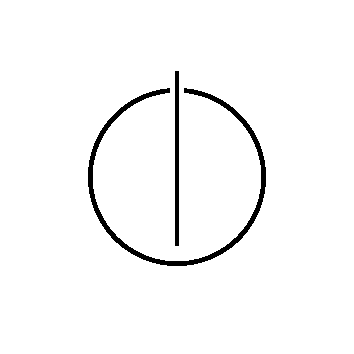
\includegraphics[width=4cm]{InformaticsLogo}
\end{figure}

\end{center}

\thispagestyle{empty}

\vspace{8mm}
\begin{center}
\oTUM{4cm}

\vspace{5mm}     
\huge FAKULT{\"A}T F{\"U}R INFORMATIK\\ 
\vspace{0.5cm}
\large DER TECHNISCHEN UNIVERSIT{\"A}T M{\"U}NCHEN\\
\end{center}

\vspace{5mm}

\begin{center}
{\Large \doctype\ in \faculty}
\vspace{8mm}

\begin{spacing}{1.3}
{\LARGE \title}\\
\vspace{8mm}

{\LARGE \titleGer}\\
\vspace{8mm}
\end{spacing}

\begin{tabular}{ll}
\Large Author:     & \Large \author     \\[2mm]
\Large Supervisor: & \Large \supervisor \\[2mm]				
\Large Advisor:	   & \Large \advisor    \\[2mm]
\Large Date:       & \Large \date
\end{tabular}

\vspace{1mm}

\begin{figure}[hb!]
\centering
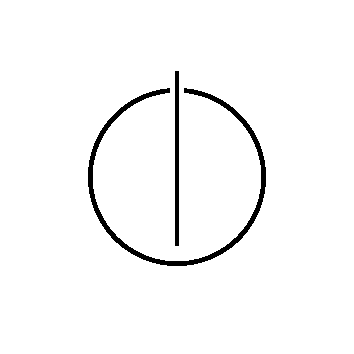
\includegraphics[width=4cm]{InformaticsLogo}
\end{figure}

\end{center}
\newpage
\thispagestyle{empty}
\mbox{}
\clearpage
\thispagestyle{empty}
\vspace*{0.8\textheight}
\noindent
I assure the single handed composition of this master thesis only supported by declared resources,

\vspace{15mm}
\noindent
Munich, \date \hspace{\stretch{1}} \author
\newpage



\newpage
\thispagestyle{empty}
\mbox{}

\chapter*{Acknowledgements}


\pagenumbering{roman}

\selectlanguage{english}
\begin{abstract}

Recent advances in Convolutional Neural Networks (CNN) have been able to conquer Computer Vision tasks and even surpass human performance. CNN algorithms are characteristically data-hungry, and obtaining domain-specific labeled data is often a cumbersome manual resource-heavy task. In this text we explore the use of synthetic data to train a CNN to perform image classification of different fasteners.

\textit{Note:}

\textit{\textbf{1. paragraph:} What is the motivation of your thesis? Why is it interesting from a scientific point of view? Which main problem do you like to solve?}

The motivation for my thesis stems from CNN algorithms' hunger for labeled images in order to train for classification tasks and produce performant results. Obtaining a large corpus of labeled images is a difficult task, especially when we wish to train a network to classify a domain-specific dataset.

\textit{\textbf{2. paragraph:} What is the purpose of the document? What is the main content, the main contribution?}
In this document we explore the use of synthetic images to augment the training data for a given CNN. We explore the power of synthetic data to produce acceptable results while using as little real data as possible. The intuition comes from the ease of rendering a large synthetic dataset on demand.

\textit{\textbf{3. paragraph:} What is your methodology? How do you proceed?}
We explore the ratio of synthetic to real images that can be used for training a CNN and obtain good results.

\end{abstract}

\clearpage

\selectlanguage{english}

\tableofcontents
\clearpage

\pagenumbering{arabic}

\fancyhead{}
\pagestyle{fancy}
\fancyhead[LE]{\slshape \leftmark}
\fancyhead[RO]{\slshape \rightmark}
\headheight=15pt

\chapter{Introduction}\label{ch:introduction}

Aircraft engine overhaul is the process of removing, disassembling, inspecting, repairing, cleaning, reassembling and testing a used engine. Overhaul involves the intricate process of taking an engine apart, and in doing so, undoing up to thousands of small parts from the engine—eg. screws, nuts and bolts. In order to reassemble the engine in the overhaul process, the small parts have to be sorted and classified. Figure \ref{fig:unclassified_small_parts} shows an example of the small parts that need to be classified.

\begin{figure}[H]
\centering
\makebox[\textwidth][c]{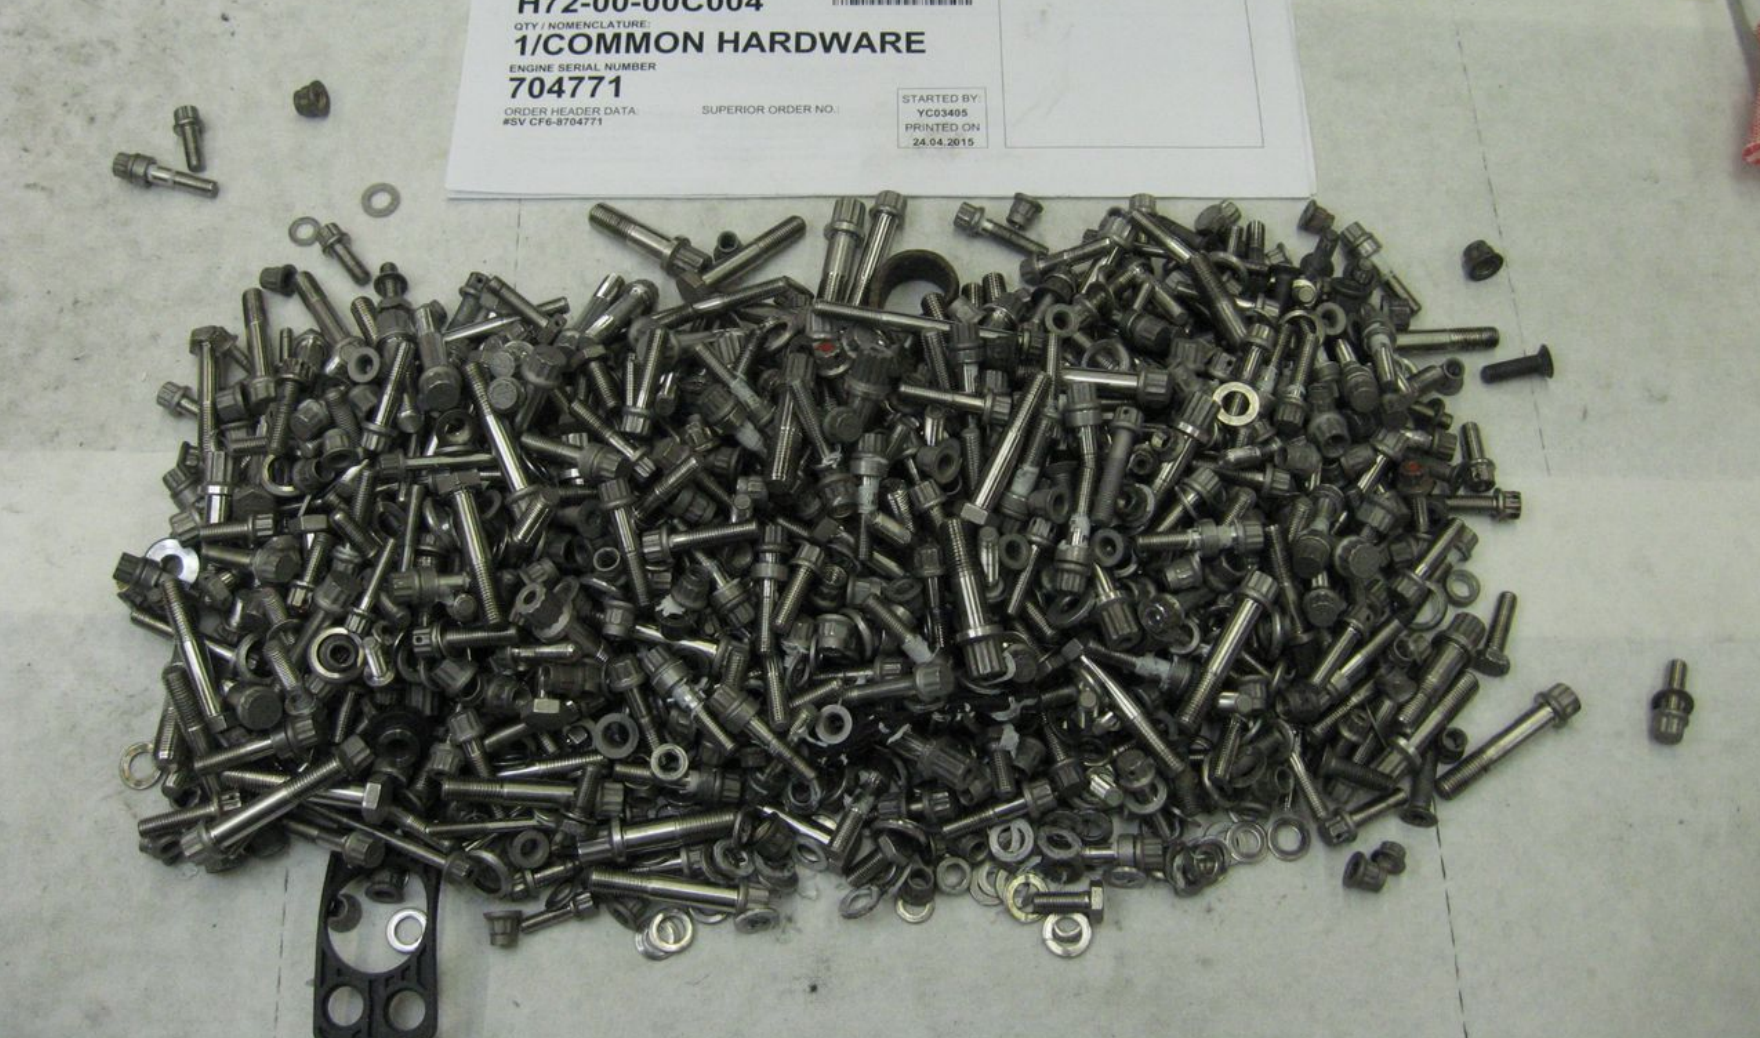
\includegraphics[width=0.65\textwidth]{unclassified_small_parts}}
\caption{Small parts that were taken apart during an aircraft engine overhaul, and have to be sorted for reassembling.}
\label{fig:unclassified_small_parts}
\end{figure}

\subsubsection{Manual Small Part Classification}

Traditionally, the tasks of classifying and sorting small parts are executed manually by a human task force. The dismantled small parts are brought to the workers in a special work station, where the workers have access to manuals, pictures of each small part, magnifiers and measuring instruments. The small parts are engraved with a part number which can be used for identification. However, sometimes the part number is indistinguishable due to erosion, rust or physical damage. In this case, the workers have to look up the small part in the manuals. The measuring instruments are used to compute the small part's distinguishing features as shown in \ref{fig:small_part_structure}. For classifying a small part with a distorted part number, the workers might need seconds to measure the different small part features and compare them against the models in the manual for classification.

\begin{figure}[H]
\centering
\makebox[\textwidth][c]{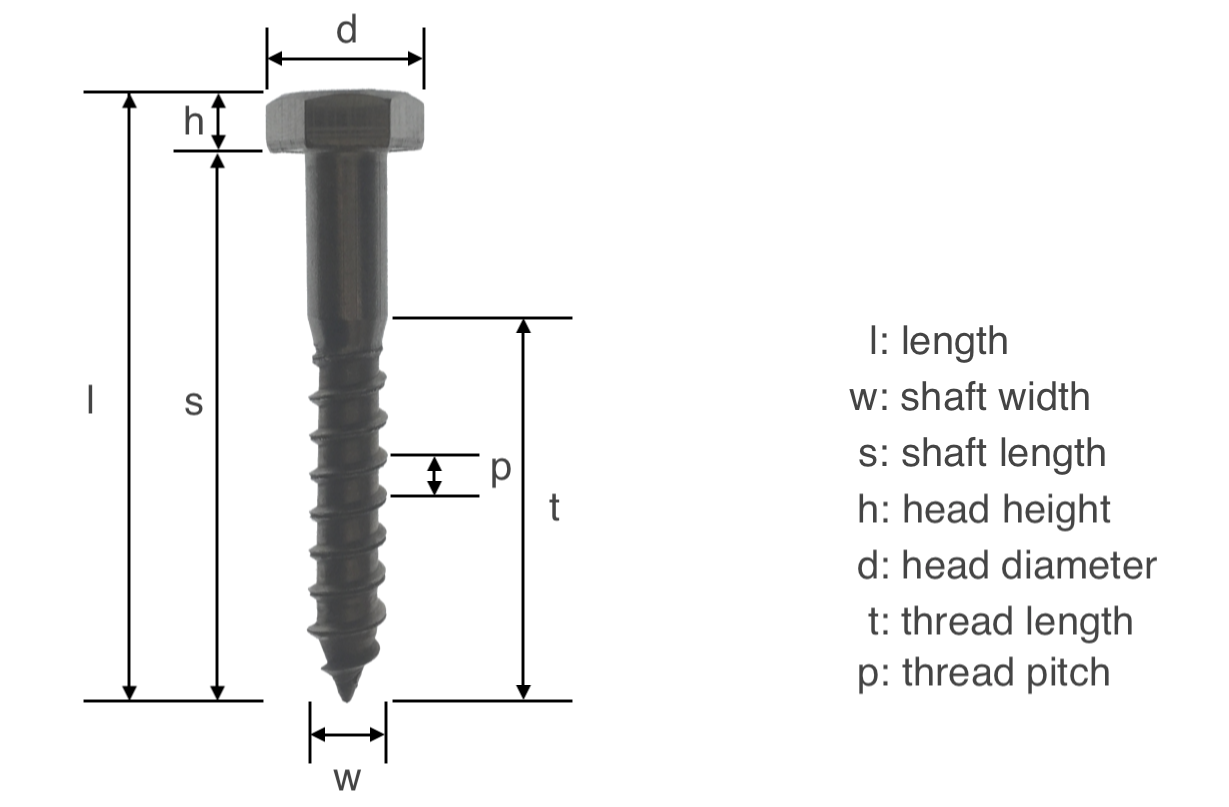
\includegraphics[width=0.85\textwidth]{small_part_structure}}
\caption{The structure of a sample screw displaying the different associated measurements.}
\label{fig:small_part_structure}
\end{figure}

\subsubsection{Automatic Small Part Classification}

An automatic small part classification system involves a setup where a camera and a robotic arm are placed over a conveyor belt. First, the small parts are placed on the conveyor belt. Next, the camera takes pictures of the small parts that are rolling underneath on the conveyor belt. The pictures are then sent to an image classification system which in turn classifies the images of the small parts. The classification system sends the labels of the small parts to the robotic arm, which uses those labels to sort the small parts accordingly. Figure \ref{fig:automatic_system} shows the automatic small part classification system.

The main brain behind automatic small part classification is the image classification system. In order to build a small part image classification system, we employ convolutional neural networks (CNNs). CNNs have become the state-of-the-art approach to classical computer vision and image processing tasks such as image classification, object detection and many others \cite{ILSVRC15}.

The automatic approach involves minimal human interaction, and thus slashes the amount of man power required to sort and classify small parts. Moreover our automatic approach provides a quantifiable measurement for accuracy which can be used to assess and improve the system.

\begin{figure}[H]
\centering
\makebox[\textwidth][c]{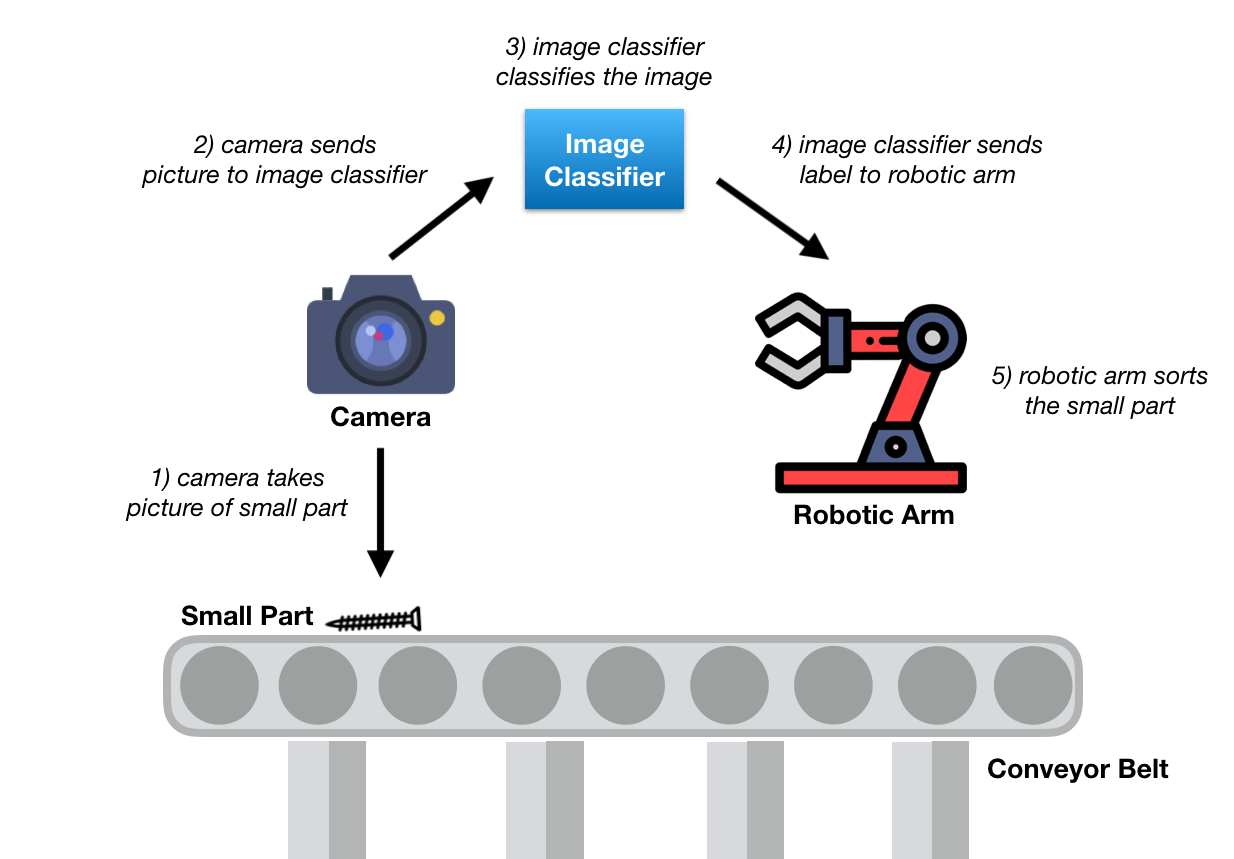
\includegraphics[width=0.9\textwidth]{automatic_system}}
\caption{The automatic small part classification system.}
\label{fig:automatic_system}
\end{figure}


\section{Problem}

Convolutional neural networks are characteristically data-hungry algorithms. The performance of a CNN algorithm depends on the availability of a dataset of images that can capture each target object's intra-class variability \cite{krizhevsky2012imagenet}. In our case, we need to train a convolutional neural network using images that capture the distinguishing features of each of our small parts. Since aircraft engines can have up to thousands of small parts, and our CNN requires multiple images of each small part, the task of collecting an image set can be time consuming.

Our contribution in this thesis is twofold. 1) we describe a system to generate synthetic images for the classification of small parts. In addition to using pictures of the small parts, we obtain their respective 3D models and use 3D modeling software to render 2D synthetic images of the small parts. The advantage being that the images are rendered rather than collected manually using a camera, and hence generation of the output image set requires less time and effort. 2) we train a convolutional neural network using synthetic images. We assess the use of synthetic data as input for CNN algorithms to perform image classification. We explore the use of a fully synthetic dataset and also a mixed dataset of both real and synthetic images in different ratios.

\section{Motivation}

Using synthetic images to classify small objects yields the power of convolutional neural network while overcoming the need to collect and annotate a dataset of images manually. This approach is extendable to image classification problems in other novel domains.

Furthermore, the process of generating synthetic images gives full control of the surrounding environment to the creator of the synthetic scene. The 3D models and the synthetic scenes can be easily adjusted to capture specific differentiating features of the small parts.

\section{Outline}
In chapter \ref{ch:background}, convolutional neural networks are described and the necessary mathematical background needed to navigate this thesis is provided. We also define the terminology that we use to describe small parts and different types of images in our dataset. Chapter \ref{ch:related_work} transcribes the literature that was reviewed in preparation for this thesis. A review of convolutional neural networks based image classification, image classification in industrial use cases and the usage of synthetic data is provided. In chapter \ref{ch:analysis}, the requirements of our system are broken down. The system use cases, object model and deployment diagrams are presented. In chapter \ref{ch:system_design}, we describe our subsystems and the relationships between them. We also describe the software and hardware components used for implementation. Chapter \ref{ch:object_design} provides an in-depth explanation of the external frameworks, APIs, algorithms and software that we use out-of-the-box. Chapter \ref{ch:evaluation} contains our implementation details, experiment design and results. Lastly, chapter \ref{ch:summary} contains a recap of our work, the conclusions we have reached and the potential future work that can be based on our thesis.

\chapter{Background}\label{ch:background}
In this chapter we provide the background needed for different concepts that are discussed in this thesis. In section \ref{sec:cnn} we introduce convolutional neural networks and how they are trained. Moreover we define the necessary terminology and provide the mathematical background required to navigate this thesis. Section \ref{sec:synth} provides the terminology that we use throughout this thesis to describe small parts, synthetic images and real images.


\section{Convolutional Neural Networks}\label{sec:cnn}
A \textbf{neural network} is a massively parallel distributed processor made up of single processing units, which has a natural propensity for storing experiential knowledge and making it available for use \cite{haykin1994neural}. Convolutional neural networks are a special type of neural network. They are typically used to solve computer vision problems like image classification and object recognition.

Regular neural networks consist of an \textbf{input layer}, \textbf{hidden layers} and an \textbf{output layer}. Every layer is made up of a set of \textbf{neurons}, where each neuron is fully connected to all neurons in the layer before. A neuron which has an input $x$ of size $n$ calculates the weighted sum $z$ as follows: \[ z = \sum_{i=1}^n w_ix_i + b_i \] where $w$ is called \textbf{weight} and $b$ is called \textbf{bias}. The weights and biases of all the neurons in a network are called the network \textbf{parameters}. Each neuron calculates its ouput $y$ by applying a differentiable non-linear function $\varphi(\cdot)$, called the \textbf{activation function}, to the weighted sum of its input signals $z$. \[y = \varphi(z)\] A neural networks relays the output of its neurons through a series of hidden layers. Finally, the last fully-connected layer, called the output layer, computes the predictions of the neural network. Figure \ref{fig:NN} shows an example structure of a regular neural network.

\begin{figure}[H]
\centering
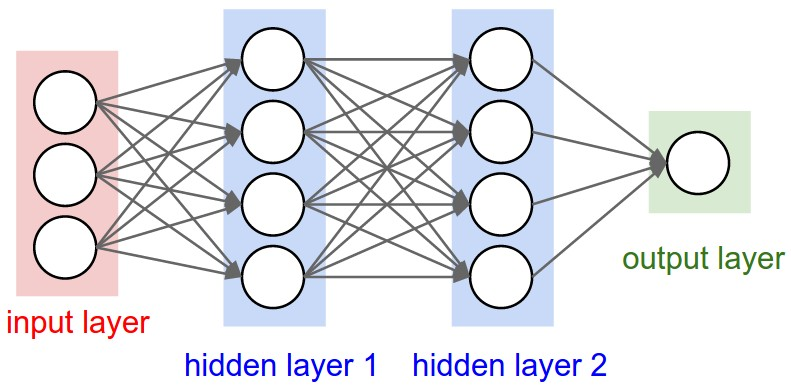
\includegraphics[width=0.75\textwidth]{NN}
\caption[A neural network with an input layer, two hidden layers and an ouput layer. Each neuron is fully connected to all the neurons in the preceeding layer.]{A neural network with an input layer, two hidden layers and an ouput layer. Each neuron is fully connected to all the neurons in the preceeding layer.\footnotemark}
\label{fig:NN}
\end{figure}
\footnotetext{Image: http://cs231n.github.io/convolutional-networks/}

Convolutional neural networks (CNNs) are structured differently. CNNs have 3 types of layers: \textbf{convolution layers}, \textbf{pooling layers} and \textbf{fully connected} layers. Convolution layers slide a weighted matrix (called \textbf{filter} or \textbf{kernel}) over the previous layer, and calculate the sum of products. The size of the step that the filter takes while sliding is called a \textbf{stride}. Figure \ref{fig:CONV} shows how a convolution layer applies a 3x3 filter to the previous layer. A non-linear activation function is applied to the output of the convolution operation to create a \textbf{feature map}. It is common to add a pooling layer after the convolution layer for subsampling, which reduces the convolution layer dimentionality. A frequently used type of pooling is \textbf{max pooling} \cite{weng1992cresceptron}. Max pooling divides the input layer into sections and computes the maximum activation of each section. Figure \ref{fig:MP} shows how a max pooling layer applies a 2x2 filter to the preceding layer. Fully connected layers are similar to layers in a regular neural network. Each neuron in a fully connected layer is connected to all neurons in the previous layer.

Figure \ref{fig:lenet5} shows the Lenet-5 convolutional neural network, which was designed by LeCun et al. \cite{lecun1998gradient} for handwritten digit recognition. Lenet-5 is an example of a CNN \textbf{architecture}. A CNN architecture is a set up of different types of layers which are combined to predict the class of the input image.

\begin{figure}[H]
\centering
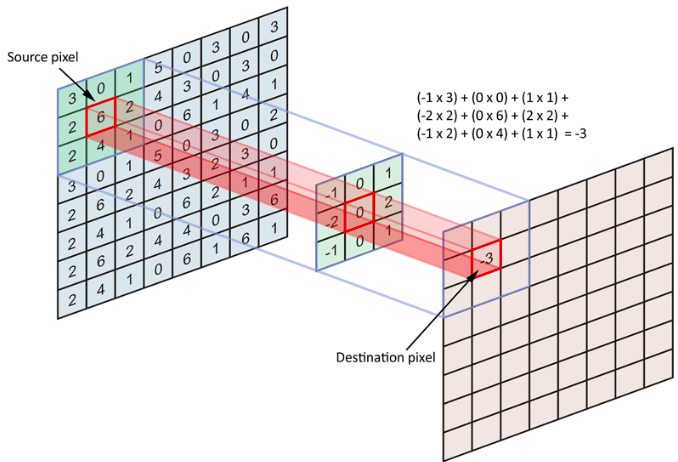
\includegraphics[width=\textwidth]{CONV}
\caption[A 3x3 filter is applied to the source pixel. Each weight in the filter is multiplied by the source's neighbouring pixel in the corresponding position. The sum of products is used to calculate the destination pixel's value in the output feature map.]{A 3x3 filter is applied to the source pixel. Each weight in the filter is multiplied by the source's neighbouring pixel in the corresponding position. The sum of products is used to calculate the destination pixel's value in the output feature map.\footnotemark}
\label{fig:CONV}
\end{figure}
\footnotetext{Image: https://towardsdatascience.com/applied-deep-learning-part-4-convolutional-neural-networks-584bc134c1e2}

\begin{figure}[H]
\centering
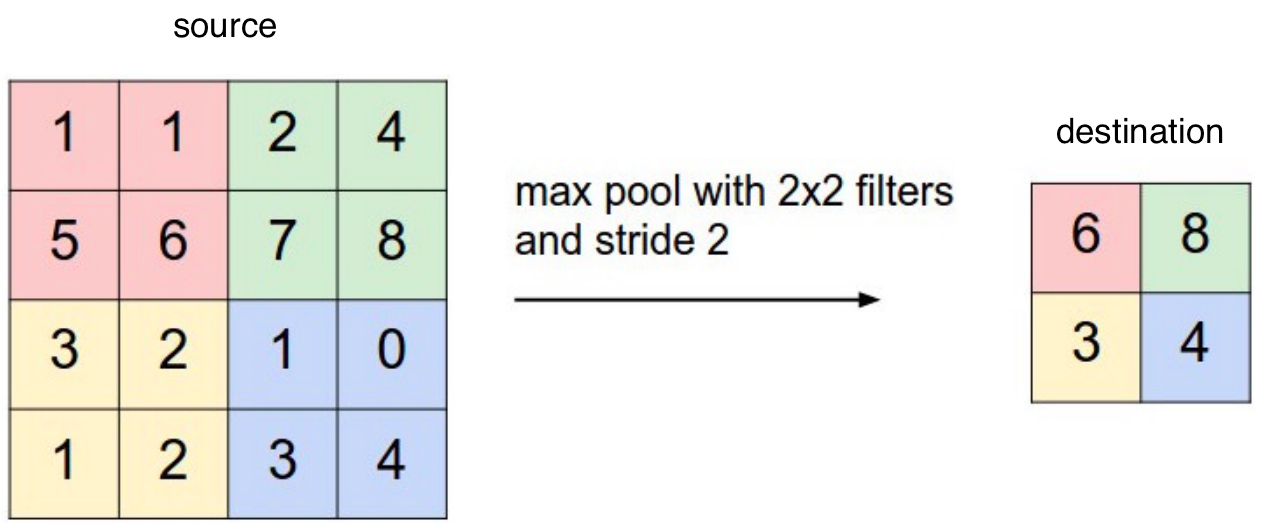
\includegraphics[width=0.7\textwidth]{MP}
\caption[A max-pooling filter of size 2x2 and stride 2 is applied to the source feature map. The maximum value of each filter is used in the destination feature map.]{A max-pooling filter of size 2x2 and stride 2 is applied to the source feature map. The maximum value of each filter is used in the destination feature map.\footnotemark}
\label{fig:MP}
\end{figure}
\footnotetext{Image: http://cs231n.github.io/convolutional-networks/}

\begin{figure}[H]
\centering
\makebox[\textwidth][c]{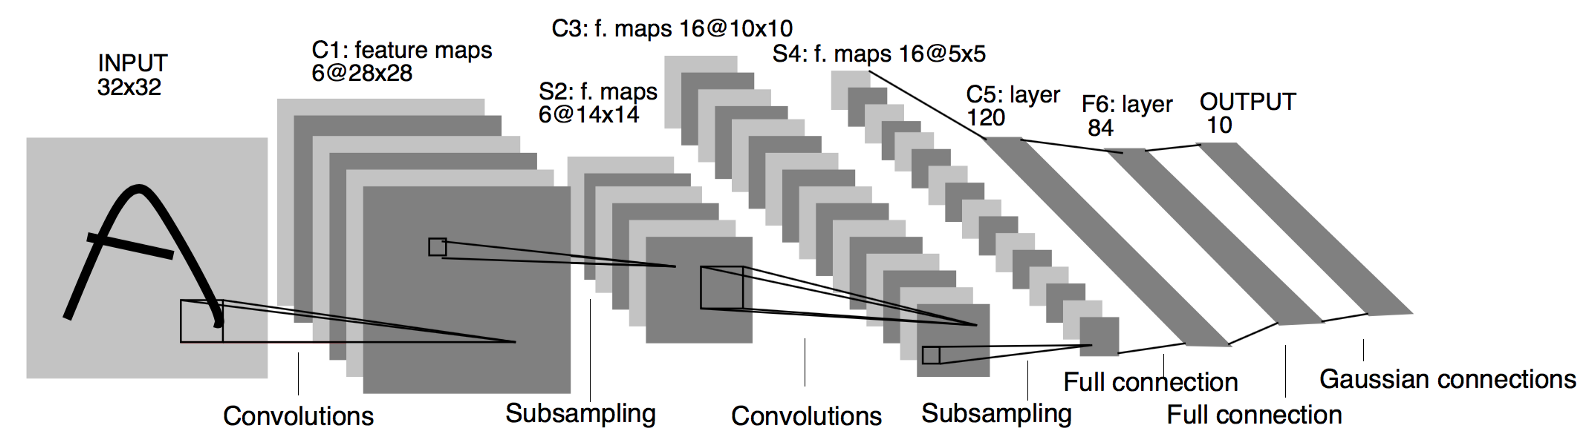
\includegraphics[width=1.3\textwidth]{lenet5}}
\caption[Architecture of the Lenet-5 convolutional neural network.]{Architecture of the Lenet-5 convolutional neural network.\cite{lecun1989backpropagation}}
\label{fig:lenet5}
\end{figure}

The Lenet-5 network uses 3x3 filters with a stride of 1 for convolution layers and 2x2 filters with a stride of 2 for subsampling layers. Lenet-5 uses \textbf{average pooling}, which calculates the average of the values in the filter.

The network takes a 32x32 image as input. The first layer is a convolution layer (C1), which applies 6 filters, followed by a subsampling layer (S2). Next comes another convolution layer (C3) which applies 16 filter, followed by a subsampling layer (S4). A final convolution layer (C5) that applies 120 filters follows S4. Afterwards comes a fully connected (F6) layer with 84 neurons. Finally, an output layer of size 10 is connected to F6. Each neuron in the output layer corresponds to the probability of the input image to be one of the 10 digits (0-9).

\subsection{Training a Convolutional Neural Network}
We train a CNN using supervised learning. Supervised learning entails that our network learns from examples. The network is presented with a \textbf{dataset} of images. The dataset is divided into a \textbf{training set}, a \textbf{validation set} and a \textbf{testing set}. Each set contains images and their corresponding \textbf{labels} (also refferd to as \textbf{classes}). We train a CNN to predict the labels of images as seen in the training set. The validation set is used for intermediate assessment of the CNN performance during the training phase, while the testing set is used to assess the performance of the CNN after the training phase is done.

CNNs process the training set in \textbf{mini-batches}. While the use of large mini-batches increases the available computational parallelism, small batch training has been shown to provide improved generalization performance \cite{masters2018revisiting}. It is also common for CNNs to process the whole training set multiple times. Each single iteration through the training set is called an \textbf{epoch}. The batch size and number of epochs are examples of CNN \textbf{hyperparameters}. Hyperparameters are network parameters that are not learnable, but rather optimized manually.

Training a convolutional neural network is the process of learning the right parameters (filter weights) to compute the correct labels from the input images in the training set. To do so, each CNN has a \textbf{loss function}. A loss function calculates the error of the predictions made by the CNN. The loss of a CNN which predicts an output \textit{y} on a training set that has the correct labels $\hat{y}$ is calculated as follows: \[L(y, \hat{y}) = \dfrac{1}{m}\sum_{i=1}^m \mathscr{L}(y_i, \hat{y}_i)\] where \textit{m} is the number of examples in the training set, and $\mathscr{L}(\cdot)$ is a distance function that calculates the difference between pairwise instances in $y$ and $\hat{y}$.

An \textbf{optimization function} (or \textbf{optimizer}) uses \textbf{back propagation} \cite{lecun1989backpropagation} to minimize the loss of a CNN during the training phase. The optimizer propagates the output of the loss function backwards by calculating the partial derivative of the loss function with respect to weights and using it to update the values of the weights.

The \textbf{stochastic gradient descent (SGD)} optimizer updates the weights of a CNN that uses the loss function $L$ thusly: \[w_{new}=w_{old}-\alpha\dfrac{\partial L}{\partial w_{old}}\] where $\alpha$ is called the \textbf{learning rate}. The learning rate controls how fast the weights are updated during training. The learning rate is a tricky hyperparameter to tune. If it is too large, the optimizer might overshoot the optimum parameter values. If it is too small, the optimizer might never reach the optimal value.

\textbf{Transfer learing} \cite{pan2010survey} is sometimes employed to speed up the training of convolutional neural networks. Transfer learning involves pre-training a CNN on images from a different domain, and then retraining the network on an image set that is specific to the desired classification task. The advantage of transfer learning is the ability to learn features from a different dataset. This is useful when we have a classification task in one domain of interest, but we only have sufficient training data in another domain. A common technique is to freeze the weights of earlier layers while training a CNN, meaning that the weights are set to be untrainable. The number of \textbf{frozen layers} is a network hyperparameter.


\section{Small Part Classification}\label{sec:synth}
We describe a system for the automatic classification of \textbf{small parts} in aircraft engines. Small parts refer to the fasteners used to build the engine like screws, bolts and nuts.

There is a set of classification challenges that are specific to small parts. A number of small parts can only be separated by subtle distinctions. This difference can be a slight change in size, which means that small parts, unlike scale invariant categories, are sensitive to differences in size, length and width. Figure \ref{fig:similar_small_parts} shows 2 screws that are identical except for a 6mm difference in length.

\begin{figure}[h]
\centering
  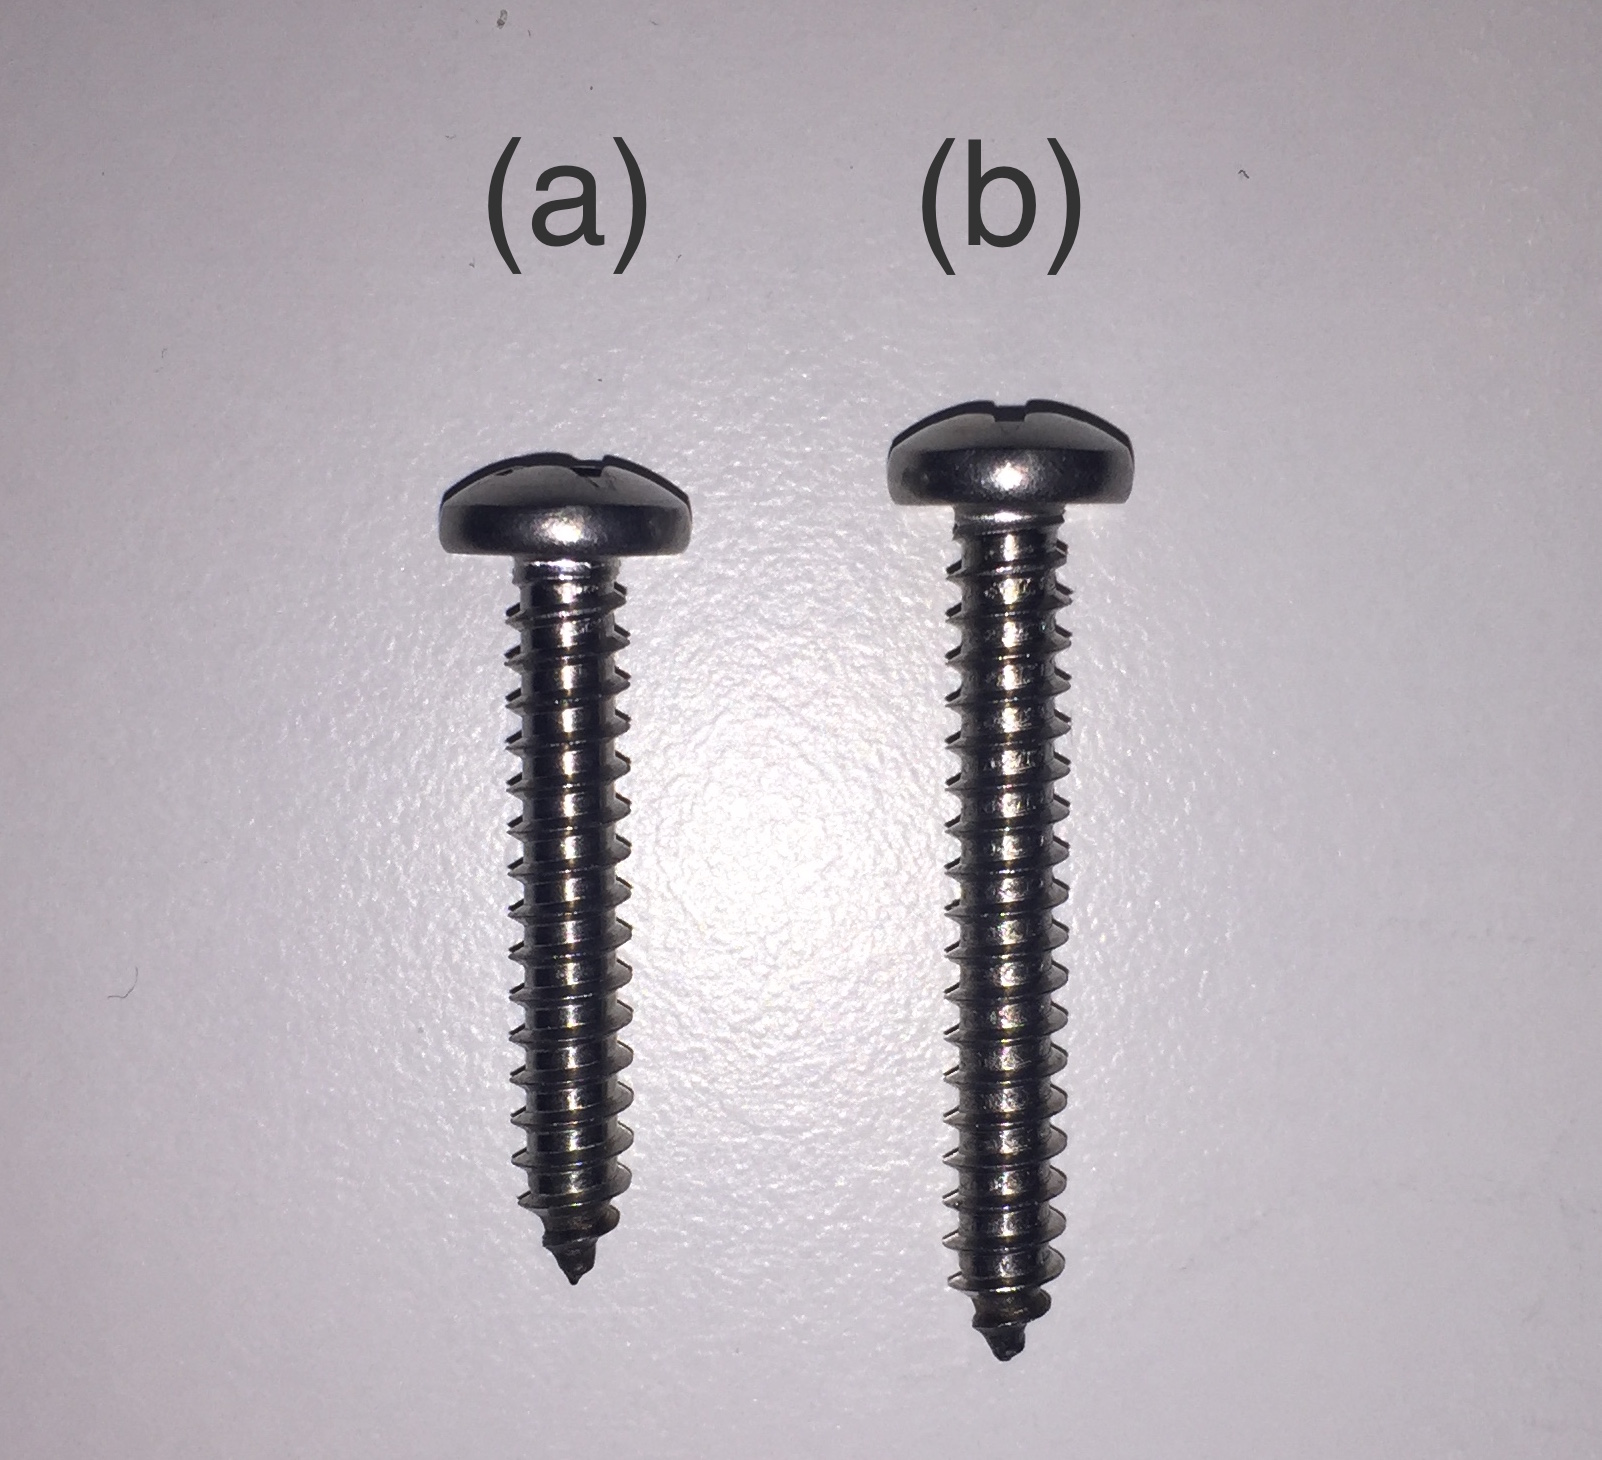
\includegraphics[width=0.5\textwidth]{similar_small_parts}
\caption{Screw (a) is identical to screw (b) except that screw (a) is 6mm shorter than screw (b). An overhead light shines on the 2 screws. The reflection changes the natural color of their surface.}
\label{fig:similar_small_parts}
\end{figure}

Aircraft fasteners are metalic and have a shiny surface. The light reflection off the fastener surface disturbs the natural surface color as shown in figure \ref{fig:similar_small_parts}, and may hide important features. Furthermore, the effect of the light reflection depends on the direction of the light, which may cause variance between images of a single small part.

Unlike cases where the background can provide information, the background is non-informative to the classification of small parts. Additionally, exposure to a regular lighting condition, like an overhead light in a room, causes the fasteners to cast a shadow on their background. A fastener shadow is not a discriminative feature. Both the background and the fastener shadow are a source of noise for the classifier.

\subsection{Real and Synthetic Images}
To automatically classify small parts, we build a convolutional neural network that is trained on both \textbf{real images} and \textbf{synthetic images}. We define real images as the natural images of the small parts, taken using a camera. Synthetic images, on the other hand, are artifically created images. They are 2-dimensional renditions of \textbf{3d models} of small parts. To generate synthetic images, we must create a \textbf{synthetic scene}: an artifical environment created in 3D modeling software. Figure \ref{fig:synthetic_scene} shows an example of a synthetic scene. A 3d model is placed in a synthetic scene in 3D modeling software. The software renders a 2D image of the environment to create a synthetic scene.

The real and synthetic images should capture the small parts and their corresponding 3D models from different angles and in different positions. To do so, we apply \textbf{transformations} to the small parts and 3D models. There are two types of trnasformations: \textbf{translation} to change the position of the target object, and \textbf{rotation} to change the angle. Each transformation has a range. This prevents the target objects from being translated or rotated away from the camera view.

\begin{figure}[h]
\centering
  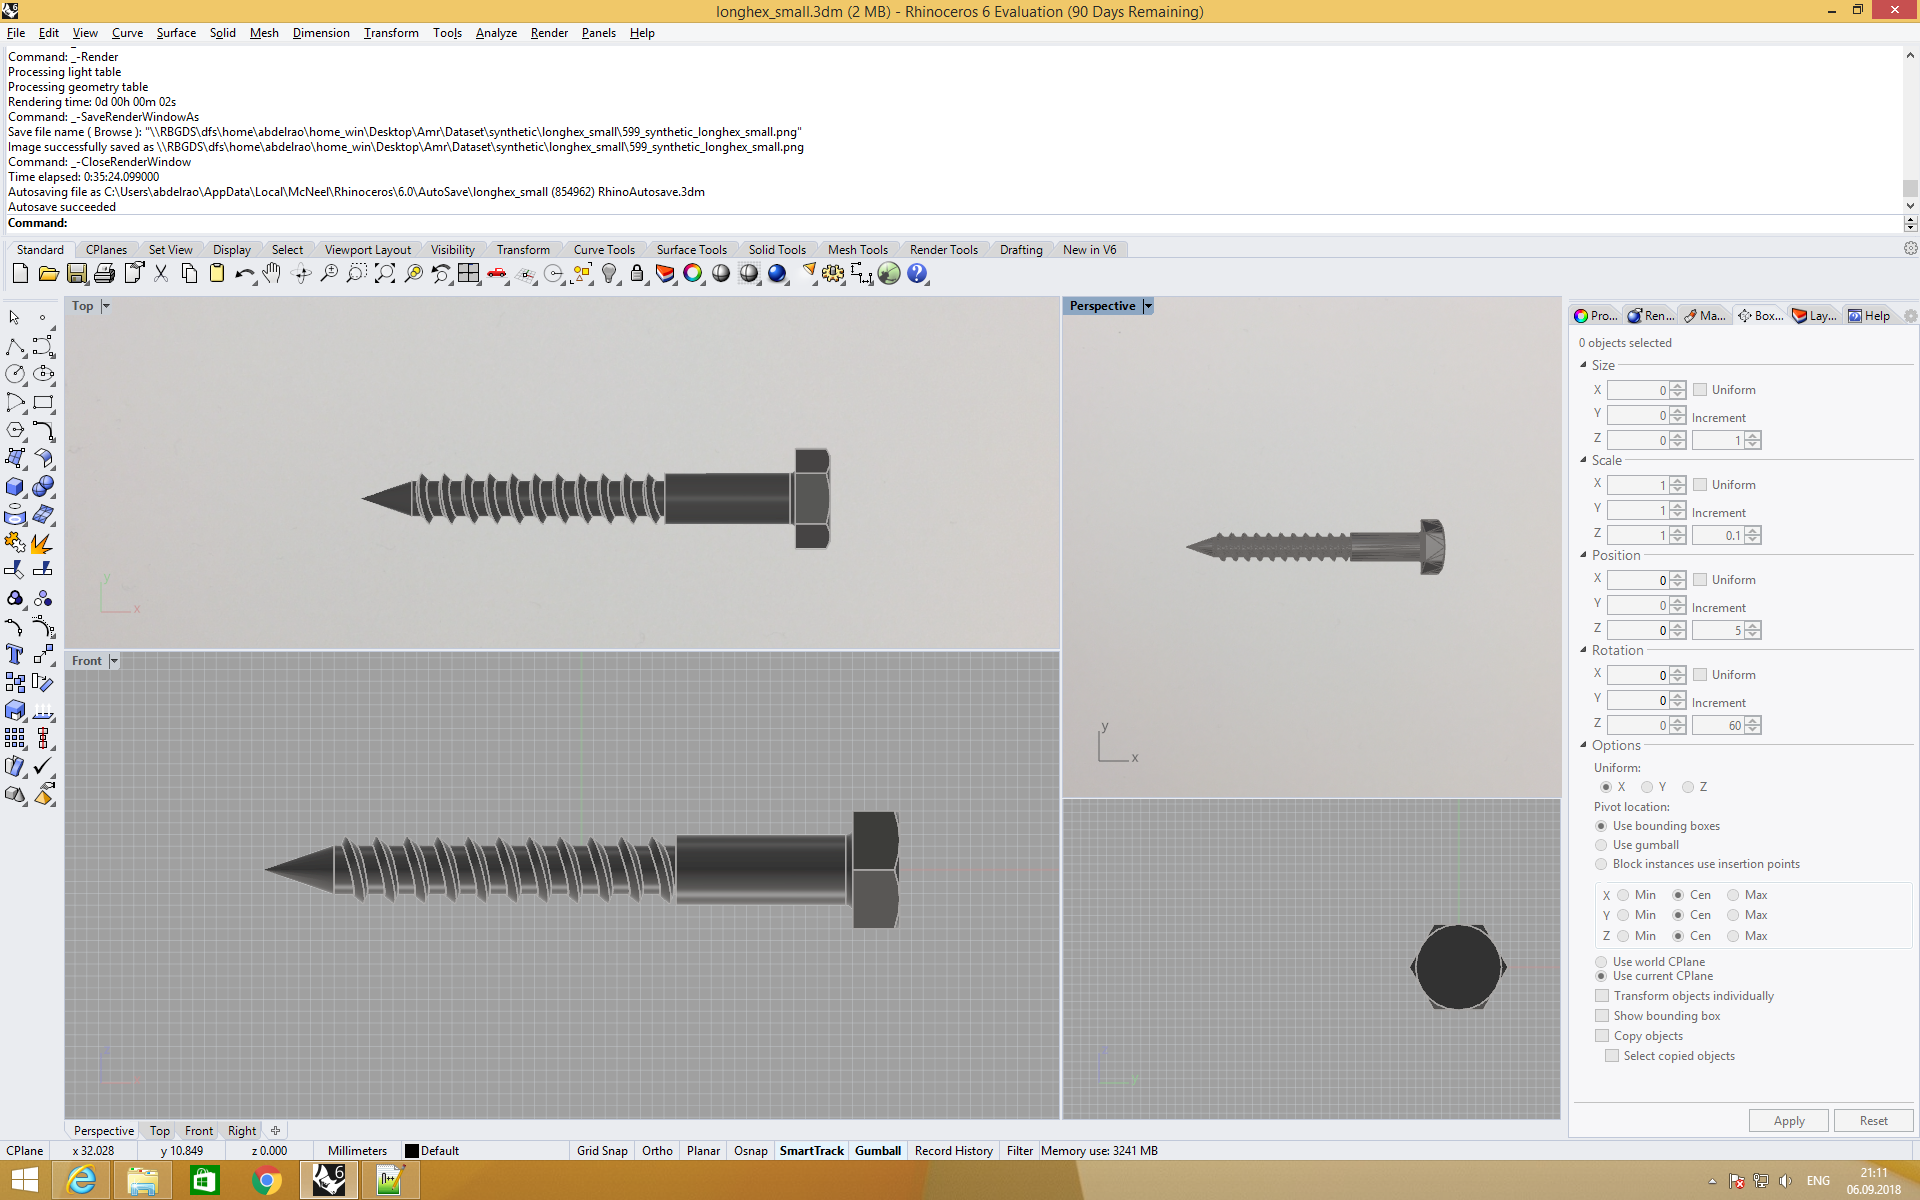
\includegraphics[width=\textwidth]{rhino_screenshot}
\caption{Synthetic scene in Rhino. The 3D model rests horizontally on a backlit plane to mimic the environment of the real setup. Sections (a) and (b) of the image depict the top view of the scene.}
\label{fig:synthetic_scene}
\end{figure}

\chapter{Related Work}\label{ch:related_work}

We provide in this chapter the literature review about topics which touch different aspects of our work. Section \ref{cnn} discusses CNN based image classification, inspired by the overview of deep learning in neural networks presented by Schmidhuber \cite{schmidhuber2015deep}. Section \ref{industrial} provides an overview of different industrial use cases of image classification. Finally, in section \ref{industrial} we examine the use of synthetic images for different computer vision problems.


\section{CNN Based Image Classification}\label{cnn}

The \textit{Neocognitron}, introduced by Fukushima \cite{fukushima1980neocognitron}, is the first neural network that resembles the modern convolutional neural network. It was based on the neurophysical insights of Hubel et al. \cite{hubel1959receptive} \cite{hubel1962receptive}, where simple cells and complex cells were observed to respond differently to stimulation in the cat’s visual cortex. Subsequently, Fukushima introduced \textit{S-cells} (corresponding to simple cells), where a weighted filter is shifted accross a 2 dimensional array to produce activations of higher order, in order to detect a particular pattern (eg. edge, shape, etc..). Fukushima also introduced \textit{C-cells} (corresponding to complex cells), which are in turn wired to the output activations of a set of S-cells. C-cells are activated if any of the preceding S-cells are activated, hence they were used as subsampling layers. The Neocognitron is a multilayered network of S-cells and C-cells. The structure of a Neocognitron is similar to what we currently know as a convolutional neural network. Fukushima applied the Neocognitron to hand-written character recognition.

In 1989, LeCun et al. used the backpropagation algorithm to train a 5-layer network (dubbed \textit{LeNet-5}) \cite{lecun1989generalization} \cite{lecun1998gradient}. Similar to the Neocognitron, there are two types of layers. Convolution layers use a weighted sliding window to accross the 2-dimensional input to calculate the layer activations. On the other hand, subsampling layers calculate the average of neighbouring input activations. LeCun et al. trained LeNet-5 on 16x16 images of handwritten digits \cite{lecun1990handwritten}, and later applied this concept to develop an application for automatically reading zip codes \cite{lecun1989backpropagation}. This work also introduced the MNIST dataset, which is a database of handwritten digits \cite{lecun1998mnist}.

Inspired by the Neocognitron, Weng et al. introduced the Cresceptron \cite{weng1992cresceptron}, which adapts the same topology during training. To implement the subsampling layers, the Cresceptron uses Max-Pooling. Here, the 2-dimensional input to the subsampling layer is partitioned into smaller rectangular arrays. Each is replaced in the subsampling layer by the maximum activation value within the partition.

Traditionally, convolutional neural networks were implemented and computed on central processing units (CPU). To speed up the processing of CNNs Chellapilla et al. provided a graphical processing unit (GPU) based implementation of convolutional neural networks\cite{chellapilla2006high}. The GPU-based implementation was 4.11 times faster than the CPU-based implementation. GPUs have become more and more important for deep learning in subsequent years.

In 2011, Ciresan et al. \cite{ciresan2011flexible} described a GPU-implementation \cite{chellapilla2006high} of a CNN with max-pooling layers\cite{weng1992cresceptron}, trained using backpropagation \cite{lecun1989backpropagation}. Ciresan et al. used this to achieve superhuman visual pattern recognition performance in the IJCNN 2011 traffic sign recognition contest in San Jose, California \cite{stallkamp2011german} \cite{cirecsan2011committee} \cite{cirecsan2012multitraffic}. Ciresan et al. obtained a 0.56\% error rate, while the human performance on the test set was 1.19\%. Furthermore, Ciresan et al. achieved human-competitive performance (around 0.2\%) on MNIST handwriting benchmark \cite{cirecsan2012multimnist}.

The ImageNet Large Scale Visual Recognition Challenge is a benchmark in object category classification and detection on hundreds of object categories and millions of images \cite{ILSVRC15}. The challenge has been conducted annually from 2010 to present. In 2012, Krizhevsky et al. \cite{krizhevsky2012imagenet} used a CNN (dubbed \textit{Alexnet}) to achieve the best results on the image classification benchmark. Alexnet achieved 16.4\% classification error, a significant improvement over the 2011 winning team, which achieved 25.8\%. Zeiler and Fergus \cite{zeiler2014visualizing} won the classification challenge in 2013. They presented a network which was based on Alexnet (dubbed \textit{ZF Net}) and were able to achieve 11.6\% classification error. Based on the work of Zeiler et al. \cite{zeiler2011adaptive}, Zeiler and Fergus developed a visualization technique called \textit{Deconvolutional Network}, which projects the feature activations back to the input pixel space. 2014 saw yet another CNN-based winning system. Szegedy et al. \cite{szegedy2015going} created a network called \textit{GoogLeNet} (also known as \textit{Inception}) that achieved 6.7\% classification error. In second place during the same year, Simonyan and Zisserman \cite{simonyan2014very} reached 7.3\% using the \textit{VGG} network.


\section{Industrial Use Cases for Image Classification}\label{industrial}

Marino et al. \cite{marino2007real} \cite{de2009gpu} describe Visual Inspection System for Railway maintenance (VISyR), which detects the presence of hexagonal-headed bolts. VISyR uses two 3-layer neural networks (NN) running in parallel. The input features to the two networks are extracted using discrete wavelet transform (DWT). The first NN uses Daubechies wavelets, while the second one uses Haar wavelets. Both neural networks are trained with same examples and fined tuned using back propagation. The system signals the presence of a hexagonal-headed bolts if both networks detect its presence. 

Gibert et al. \cite{gibert2015robust} describes a method to detect the presence of a fastener in an image, determine whether the fastener is broken, and further subcategorize the fastener into one of five classes. The method uses Histogram of Gradients (HOG) to extract features, and a Support Vector Machine (SVM) for classification. In the same year, Gibert et al. \cite{gibert2015material} presented a way to classify materials in images of railway tracks. Gibert et al. use a 4-layered convolutional neural network to perform segmentation on the input images. The network classifies each pixel in the image into one of 10 materials. The CNN was trained to detect chipped or crumbling railway crossites. In 2017, Gibert et al. \cite{gibert2017deep} presented an approach to perform the tasks simultaneously: classify both the materials and the fasteners in an input image. Gibert et al. extended the material classification network \cite{gibert2015material} by extracting the features from the 3rd network layer. The features were used as input for an SVM classifier to detect the presence of a fastener and classify its type if found.

In 2015, Aytekin et al. \cite{aytekin2015railway} describe a real-time railway fastener detection system using a high-speed laser range finder camera, which is placed under a railway carriage designed for railway quality inspection. Aytekin et al. present multiple pixel-similarity-based approaches, namely principal component analysis (PCA), linear discriminant analysis (LDA), random-forest (RF), sparse representation (SR), and multitemplate matching (MTM). Moreover, the histogram-based approaches histogram matching (HM) and depth peeks (DP) approaches are also implemented. Aytekin et al. focused on false alarm rate (FAR) as an evaluation metric since they wanted to minimize false positives. Aytekin et al. concluded that a combination of PCA and DP produce the least false alarm rate.

Feng et al. \cite{feng2014automatic} describes a method to perform automatic fastener classification and defect detection. Their system which places 2 cameras under a train coach, which in turn takes pictures of the track and sends it to an onboard processor which performs fastener localization, classification and defect assessment by ranking the status of the fasteners. Feng et al. propose a novel classification technique based on Latent Dirichlet Allocation (LDA). Their system can model different types of fasteners using unlabeled data and is robust to illumination changes.


\section{Using Synthetic Images}\label{synthetic}

Synthetic images have been used for training in a variety of problems. Peng et al. \cite{peng2015learning} uses 3D CAD models to generate synthetic images. These images are then used to tests the invariance of convolutional neural networks to low level cues, namely, object texture, color, 3D pose and 3D shape, as well as background scene texture and color. Peng et al. uses RCNN \cite{girshick2014rich} to test cue invariance in object detection. 

The work done in \cite{rajpura2017object} train a CNN object detector to recognize objects inside a fridge. The work renders non-photorealistic synthetic scenes of 55 distinct products inside a fridge. The work evaluates the use of a fully synthetic training set versus a training set which includes 10\% real data.

In the same manner as \cite{rajpura2017object}, the work done in \cite{georgakis2017synthesizing} synthesizes training data for object detection in indoor scenes. The work creates synthetic data by superimposing 3D models on real scenes. The work compares purely synthetic training sets as well as different ratio of real to synthetic training images.

The work in \cite{sarkar2017trained} trains a CNN image classifier on synthetic images rendered from 3D models of 5 different objects.

The work in \cite{goyal2017dataset} uses synthetic images to perform semantic segmentation. The work renders synthetic images using 3D models. In addition, pixel-wise annotations of the synthetic images are generated. A CNN is trained on the annotated synthetic images and the intersection over union (IoU) is evaluated.
\chapter{Analysis}

%\textit{Note: This chapter follows the Requirements Analysis Document Template in \cite{bruegge2004object}. 
%\textbf{Important:} Make sure that the whole chapter is independent of the chosen technology and development platform. The idea is %that you illustrate concepts, taxonomies and relationships of the application domain independent of the solution domain!
%Cite \cite{bruegge2004object} several times in this chapter.}

\section{Overview}

Our goal is to develop a system that classifies images of different small mechanical parts (SMPs), and to do so as accurately as possible. To realize this goal, we decide to leverage state-of-the-art advancements in Convolutional Neural Network algorithms in the field of computer vision, and more specifically, the sub-field of image classification.

We aim to build a system that scales up well, ie. we would like the classification system to easily adapt new small mechanical parts. Moreover we would like to build a system that can scale up to thousends of classes.

CNN algorithms are characteristically data-hungry. The classification accuracy of a CNN algorithm is proportional to the amount of images that are fed in as input. Given the large number of classes, the task of collecting images of each small mechanical part becomes time-consuming and labour-intensive. To combat this problem, we decide to augment the training data of our algorithms with \textit{synthetic images}: 2-dimentional renditions of 3-dimensional computerized graphical models of the small mechanical parts. We hypothesize that our synthetically augmented training set will yield a higher accuracy, whilst minimizing the manual effort needed to take real images of the small mechanical parts.

\section{Requirements}

\subsection{Functional Requirements}

Functional requirements (FRs) describe the interactions between the system and the its environment independent of its implementation. \cite{bruegge2004object}.

The system's main function is to classify images of different small mechanical parts. Furthermore, the system needs to be dynamic and scalable to accomodate new small mechanical parts. To ensure that the system is able to classify images accurately, while leveraging synthetic input images, we introduce the following Functional Requirements.

\begin{itemize}
  \item [FR1] \textbf{Generate Synthetic Images}: Given a 3D model of a small mechanical part, the system should generate a set of synthetic images of said model. The system should apply a set of random transformations to the 3D model before rendering the 2D synthetic image to ensure that the generated dataset captures the SMP from as many angles in as many positions as possible.

  \item [FR2] \textbf{Add New Class to Image Classifier}: The system should accomodate the addition of a new SMP to the classifier. This extends to the ability of the system to accomodate for new input training data, and the ability to label a new output class.

  \item [FR3] \textbf{Adjust input data split}: The system should allow for changes in the training, validation and testing input data which is assigned as input to the image classifier. This includes changing the number of images in each set and manipulating the ratio of synthetic to real images in the training split.

  \item [FR4] \textbf{Retrain Image Classifier}: The system should be dynamic enough to retrain the image classifier. This step is usually taken after the augmenting or adjustment of the input data split.

  \item [FR5] \textbf{Fine-Tune Image Classifier}: The underlying CNN algorithm should be subject to fine-tuning in order to maximize the accuracy of the system.
\end{itemize}

\subsection{Nonfunctional Requirements}

Nonfunctional Requirements (NFRs) are key system requirements that apply to the system as a whole. To maintain the system's general requirements we define the following nonfunctional requirements.

\begin{itemize}
  \item [NFR1] \textbf{Performance}: A performence requirement is the measure of a quantifiable attribute of our system. In our case we would like to track our system's \textbf{classification accuracy}.\\
  We first specify our system's accuracy for a single class to be the percentage of the given class's testing image split that the image classifier correctly predicts. We consequently define our system's classification accuracy to be the image classifier's average prediction accuracy over each class.

  \item [NFR2] \textbf{Adaptability}: Adaptability is the ability to change the system to deal with additional application domain concepts \cite{bruegge2004object}. Our system needs to be dynamic enough to accomodate for new small mechanical parts that can be later added even after the system has been deployed.
\end{itemize}

\section{System Models}

\subsection{Use Case Model}

Use case models represent the relationship between the user group of a system and the general functions that they can execute. A use case model can reduce the complexity of a system and increase its understandability.

The use case model of our system can be found as figure [\ref{fig:UCM}]. The two main protagonists of our system are the data collector, who is tasked with collecting synthetic and real images, and the machine learning expert, who is responsible for training the system to classify a set of small mechanical parts.

\begin{figure}[h]
\centering
  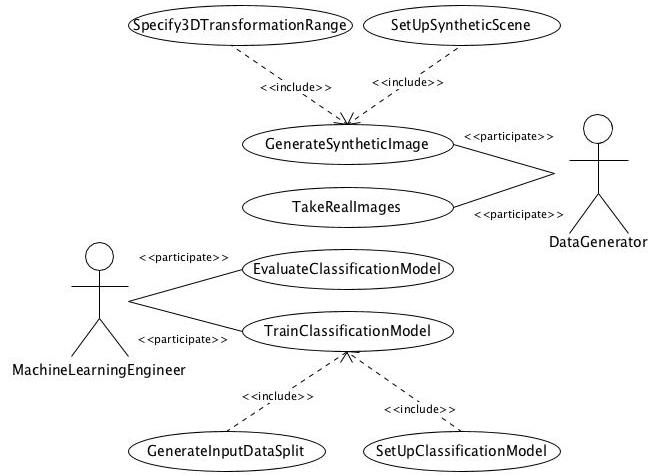
\includegraphics[width=\textwidth]{UCM}
\caption{Use Case Model}
\label{fig:UCM}
\end{figure}

The use case model can be divided into 3 main functions; namely generating synthetic images, obtaining real images, and training an image classifier.

\subsubsection{Generating Synthetic Images}

Generating synthetic images the cornerstone for a synthetically augmented dataset. There's a lot of work that goes into generating the 3D synthetic scene and the corresponding renditions. To increase the understandability of our model, we have separated the the use case that revolve around modeling the SMP 3D model itself as \textit{Specify3DModelTransformations}, and the use case that deals with the synthetic scene environment as \textit{SetUpSyntheticScene}.

\begin{usecase}
  \addtitle{Use Case}{Specify3DModelTransformations}

  \addfield{Participating Actors}{DataCollector}

  \addscenario{Flow of Events}{
    \item In the modeling software, the DataCollector chooses the transformations that are applicable to the small mechanical part's 3D model.
    \item For each transformation, the DataCollector sets the range of each tranformation attribute that will be later used to generate a random position for the synthetic image of the SMP.
  }

  \addfield{Entry Condition}{DataCollector has modeling software open.}

  \addfield{Exit Condition}{All the desired transformations and their corresponding attributes have been specified.}

  \additemizedfield{Quality Requirements}{
    \item In the effort to achieve the Performance Non-Functional requirement, synthetic images have to look as photo realistic as possible. The 3D transformations should strive to output the range of positions that the respective SMP can be placed in.
  }
\end{usecase}

\clearpage
\begin{usecase}
  \addtitle{Use Case}{SetUpSyntheticScene}

  \addfield{Participating Actors}{DataCollector}

  \addscenario{Flow of Events}{
    \item In the modeling software, the DataCollector places the 3D model of the SMP on a horizontal plane as if lying on a table.
    \item The DataCollector sets the background of the horizontal plane to mimic the background of the real images in the dataset.
    \item The DataCollector sets the lighting condition of the scene to reflect the lighting condition of the environment where the real SMP images are taken.
  }

  \addfield{Entry Condition}{DataCollector has modeling software open.}

  \addfield{Exit Condition}{In the modeling software, the 3D model of the SMP should be lying on a horizontal plane with a background and lighting condition that reflect the environment of the real SMP images.}

  \additemizedfield{Quality Requirements}{
    \item The synthetic scene should look as photorealistic as possible. This helps the Image Classifier achieve a higher classification accuracy using the synthetic images.
  }
\end{usecase}

\clearpage
\begin{usecase}
  \addtitle{Use Case}{GenerateSyntheticImages}

  \addfield{Participating Actors}{DataCollector}

  \addscenario{Flow of Events}{
    \item The DataCollector specifies the desired number of output synthetic images.
    \item The modeling software generates the desired number of output synthetic images. Each image is a rendition of the scene after the transformations have been applied to the 3D model.
  }

  \addfield{Entry Condition}{DataCollector has modeling software open.}

  \addfield{Exit Condition}{The DataCollector obtains a set of synthetic images for the specified SMP that can be later used to train the Image Classifier.}
\end{usecase}

\clearpage
\subsubsection{Obtaining Real Images}

\begin{usecase}
  \addtitle{Use Case}{TakeRealImages}

  \addfield{Participating Actors}{DataCollector}

  \addscenario{Flow of Events}{
    \item The DataCollector places the camera over a plane.
    \item The DataCollector sets the SMP over the plane in a random position, such that the full SMP body is within the viewfield of the camera.
    \item The DataCollector takes a picture of the SMP.
    \item The DataCollector repeats steps 2 and 3 until the desired number of real images of the SMP is reached.
    \item The DataCollector resizes the images to correspond to the input image size of the Image Classifier. 
  }

  \addfield{Entry Condition}{}

  \addfield{Exit Condition}{The DataCollector obtains a set of real images for the specified SMP that can be later used to train the Image Classifier.}

  \additemizedfield{Quality Requirements}{
    \item The lighting of the environment should eliminate shadows and light reflections on the SMP surface.
  }
\end{usecase}

\clearpage
\subsubsection{Training the Image Classifier}

Training the image classifier requires some underlying work. We have chosen to model this use case as one that includes setting up the input data and configuring the image classifier (modeled as \textit{SetInputDataSplit} and \textit{SetUpImageClassifier} respectively).

\begin{usecase}
  \addtitle{Use Case}{TrainImageClassifier}

  \addfield{Participating Actors}{MachineLearningEngineer}

  \addscenario{Flow of Events}{
    \item The MachineLearningEngineer configures the dataset structure: number of images for training, validation and testing, as well as the ratio of real to synthetic images in the training split.
    \item The MachineLearningEngineer chooses a convolutional neural network architecture for the Image Classifier.
    \item The MachineLearningEngineer fine-tunes the CNN by manipulating its hyperparameters.
  }

  \addfield{Entry Condition}{For each SMP set to be classified by the Image Classifier, the corresponding real and synthetic images should be generated and ready for use.}

  \addfield{Exit Condition}{The Image Classifier outputs the maximum possible accuracy given the input dataset.}
\end{usecase}

\clearpage
\subsection{Analysis Object Model}

The analysis object model is a visual dictionary of the main concepts visible to the user \cite{bruegge2004object}. The analysis object model depicts a system's entites, their corresponding attributes and functions, and illustrates the relationship between said entitie. Figure [\ref{fig:AOM}] represents the analysis object model of our system.

\subsubsection{SmallMechanicalPart}
A small mechanical part is the main subject of our system. It is an object that our system aims to classify. Each SMP has a unique identifying label string.

\subsubsection{3DModel}
A 3DModel of a small mechanical part is the graphical model which helps our system create synthetic images. Each SMP has a corresponding 3DModel. Each 3DModel has the same label as its SMP counterpart.

\subsubsection{Transformation}
Each SMP and 3DModel have a list of applicable transformations. A transformation is executed on an axis (x, y or z), and can either be a Translation or a Rotation.
At image generation time, each transformation outputs a random value between its defined maximum and minimum. We define a range to limit an object's transformation. For instance, we don't want to translate an SMP so far as to remove it from the camera's viewfield.

\subsubsection{ImageGenerator}
ImageGenerator is the class that does the heavy lifting when it comes to creating images. It applies the random transformations on the target object and generates an image with a specified width and height.
ImageGenerator is an abstraction of 2 classes. SyntheticImageGenerator is responsible for applying the transformations on 3DModels, and using SyntheticScene to generate SyntheticImages, while RealImageGenerator uses a camera to take pictures of SmallMechanicalParts and output their corresponding RealImages.

\subsubsection{Image}
Image is a generalization of RealImage and SyntheticImage. Image stores information like width, height and label of the image. Moreover it contains a dataBuffer which contains the actual image pixel values.

\subsubsection{Dataset}
Dataset is a composition of Images. It is the image repository which is used by the ImageClassifier for training and evaluation.

\subsubsection{DataSplitGenerator}
DataSplitGenerator splits the Dataset into a training set, validation set and testing set. This split prepares the data for consumption by the ImageClassifier.

\subsubsection{CNNModel}
CNNModel is the convolutional neural network algorithm that is trained for image classification. CNNModel is an abstraction of 4 different CNN architectures, namely Inception, Resnet, VGG16 and VGG19. Furthermore, CNNModel defines the weights that are used to initialize the CNN to leverage the power of transfer learning. CNNModel also sets the number of trainable layers in a network to potentially preserve the initial weights and speed up training.

\subsubsection{Optimizer}
Each CNNModel has an Optimizer. An Optimizer is the function aims to close the gap between the model's predictions of the validation set labels and their corresponding ground truth. The Optimizer operates in the CNNModel's training phase. Optimizer is an abstraction of 2 different optimizers that we use in our system. Specifically SGD (Stochastic Gradient Descent), and Adam.

\subsubsection{ImageClassifier}
ImageClassifier orchestrates the feeding of data into the CNNModel for training. Moreover, it uses the testing set to calculate the accuracy of the trained model.

\begin{figure}[H]
\centering
  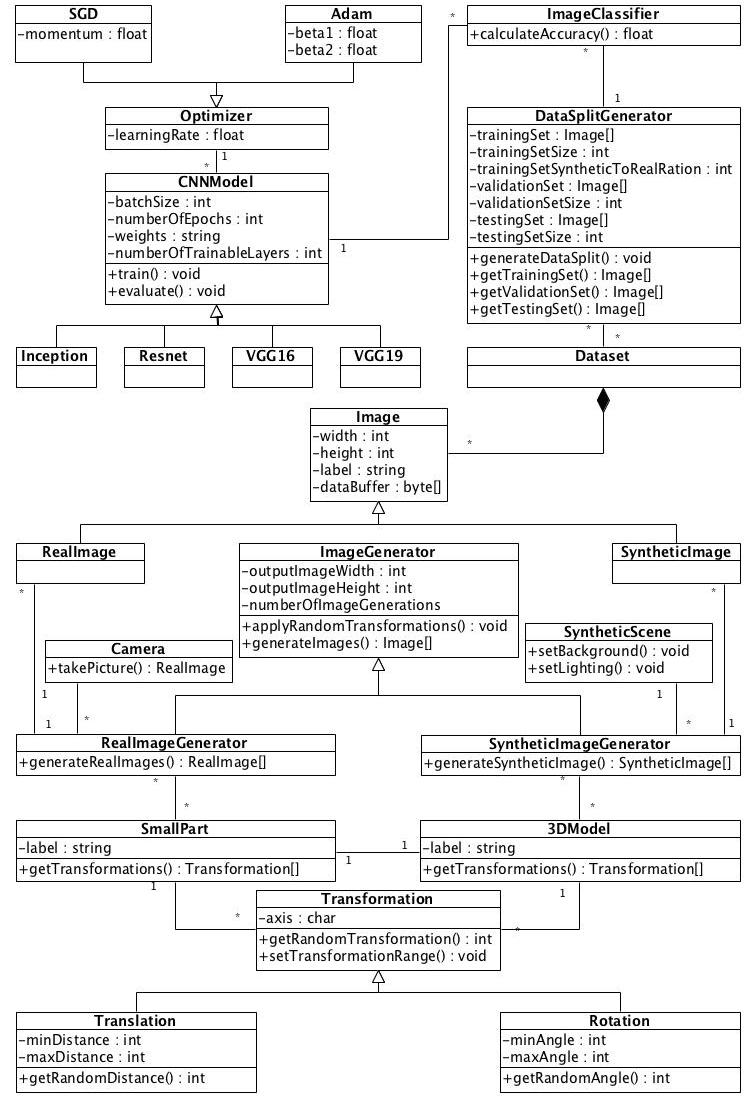
\includegraphics[width=\textwidth]{AOM}
\caption{Analysis Object Model}
\label{fig:AOM}
\end{figure}

\subsection{Dynamic Model}

The dynamic model is focused on the behavior of the system. Sequence diagrams, activity diagrams and state machines are usually used to depict dynamic models \cite{bruegge2004object}. In this section we present 2 activity diagrams that depict the 2 main workflows of our system.

\subsubsection{Dataset Generation}

Figure [\ref{fig:AD1}] depicts the workflow of activities required to generate a dataset. The DataCollector selects a small mechanical part and its corresponding 3D model. The DataCollector then proceeds to generate the real and synthetic images. Finally the images are combined to form a dataset.

\begin{figure}[h]
\centering
  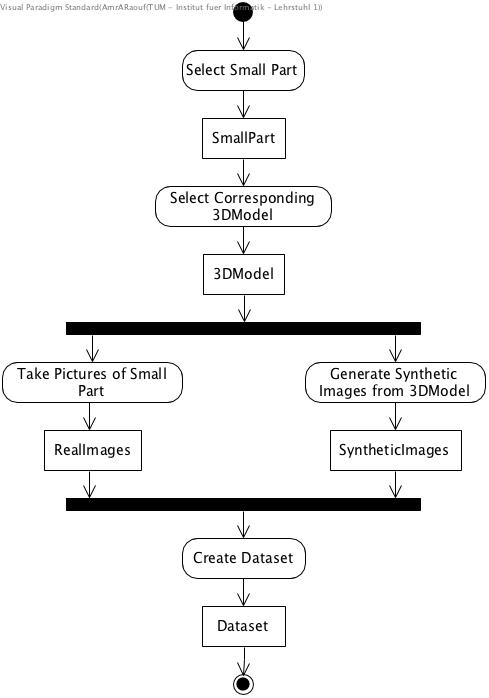
\includegraphics[width=\textwidth]{AD1}
\caption{Activity Diagram depicting the workflow required for Dataset generation}
\label{fig:AD1}
\end{figure}

\subsubsection{Training the Image Classifier}

Figure [\ref{fig:AD2}] describes the workflow of activities required to train the image classifier. The MachineLearningEngineer splits the data into training, validation and testing sets. The MachineLearningEngineer then creates a CNN model. Next the MachineLearningEngineer feeds the training data to the CNN model to obtained a trained CNN model. The MachineLearningEngineer then evaluates the trained CNN model accuracy using the testing set. If the accuracy of the trained CNN model is not sufficient, the CNN model is fine tuned and re-trained.

\begin{figure}[h]
\centering`
  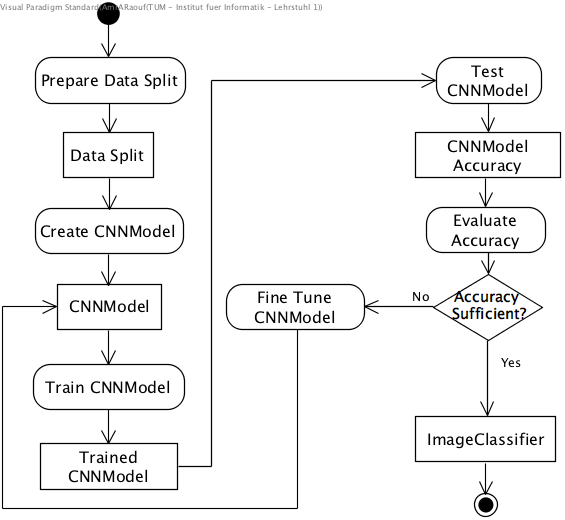
\includegraphics[width=\textwidth]{AD2}
\caption{Activity Diagram describing the workflow required to train the Image Classifier}
\label{fig:AD2}
\end{figure}

\chapter{System design}\label{ch:system_design}

In the previous chapter, we have extracted the functional and non-functional requirements of our system. Subsequently, we broke down our system into use cases in the use case model. Furthermore, we have described the entities of our system and the relationships between them using an Analysis Object Models and we presented 3 activity diagrams that depict the workflows in our system.

In this chapter we map our analysis into the solution domain. We first identify our design goals in section \ref{sec:design_goals}. In section \ref{sec:subsystem_decomposition}, we group the objects that we have identified in the analysis object models into subsystems, and we discuss the dependencies between those subsystems. In section \ref{sec:hardware_software_mapping} we present the hardware and software components used to implement our system. Lastly, section \ref{sec:persistent_data_management} presents the structure of our system's persistent data.


\section{Design Goals}\label{sec:design_goals}

In the previous chapter we have defined our non-functional requirements. In this section, we use those non-functional requirements to extract our design goals, and we use those design goals as a compass for our system design. Defining our design goals allows us to make consistent design decisions across our different subsystems. Table \ref{tab:DG} lists our non-functional requirements and their corresponding design goal. There are 5 types of possible design criteria from which the design goals can be selected: performance, dependability, cost, maintenance and end user criteria \cite{bruegge2004object}.

\begin{table}
  \centering
  \begin{tabular}{ | l | p{5cm} | l | }
    \hline
    \textbf{Requirement} & \textbf{Design Goal} & \textbf{Criteria} \\ \hline
    \textbf{Adaptability} & The system should create a convolutional neural network that can accommodate the addition of new classes. & Performance \\ \hline
    \textbf{Accuracy} & The system should utilize real and synthetic images to train a CNN model to classify different small parts with high accuracy. & Performance \\ \hline
  \end{tabular}
  \caption{Non-functional requirements and their corresponding design goals.}
  \label{tab:DG}
\end{table}


\section{Subsystem Decomposition}\label{sec:subsystem_decomposition}

Figure \ref{fig:SSD} depicts our system's subsystem decomposition. Our system is divided into 3 subsystems. \textbf{SyntheticImageSubsystem} is responsible for providing our system with synthetic images. It consists of 4 main components: \textbf{3DScanner}, \textbf{3DScanningSoftware}, \textbf{3DScanningSoftware}, \textbf{SyntheticScene} and \textbf{3DModelingSoftware}. The 3DScanner scans \textbf{SmallParts} and outputs raw 3D model, which are processes by the 3DModelingSoftware to create a \textbf{3DModel}. The SyntheticScene generates an artificial environment. The 3DModelingSoftware places the 3D models in the environment created by SyntheticScene, and renders \textbf{SyntheticImages} of the 3D models.

On the other hand, \textbf{RealImageSubsystem} is responsible for providing our system with real images. The \textbf{Camera} is used to take real images of the SmallParts. Next, the \textbf{RealImageProcessor} resizes the raw images to provide our system with \textbf{RealImages} that can be used out of the box.

The synthetic images created by the SyntheticImageSubsystem and the real images created by the RealImageSubsystem are both sent to the \textbf{ImageClassifierSubsystem}. The ImageClassifierSubsystem in turn combines both image sets to create a \textbf{Dataset}. The images are then fed to the \textbf{DatasetSplitter}, which is in turn responsible for splitting the data into a training set, a validation set and a testing set. The \textbf{ImageClassiefier} uses the training and validation sets to train a \textbf{CNNModel}. The CNNModel uses an \textbf{Optimizer} to adjust the model weights during the training phase. The testing set is then used to evaluate the accuracy of the trained CNNModel.

\begin{figure}[H]
\centering
  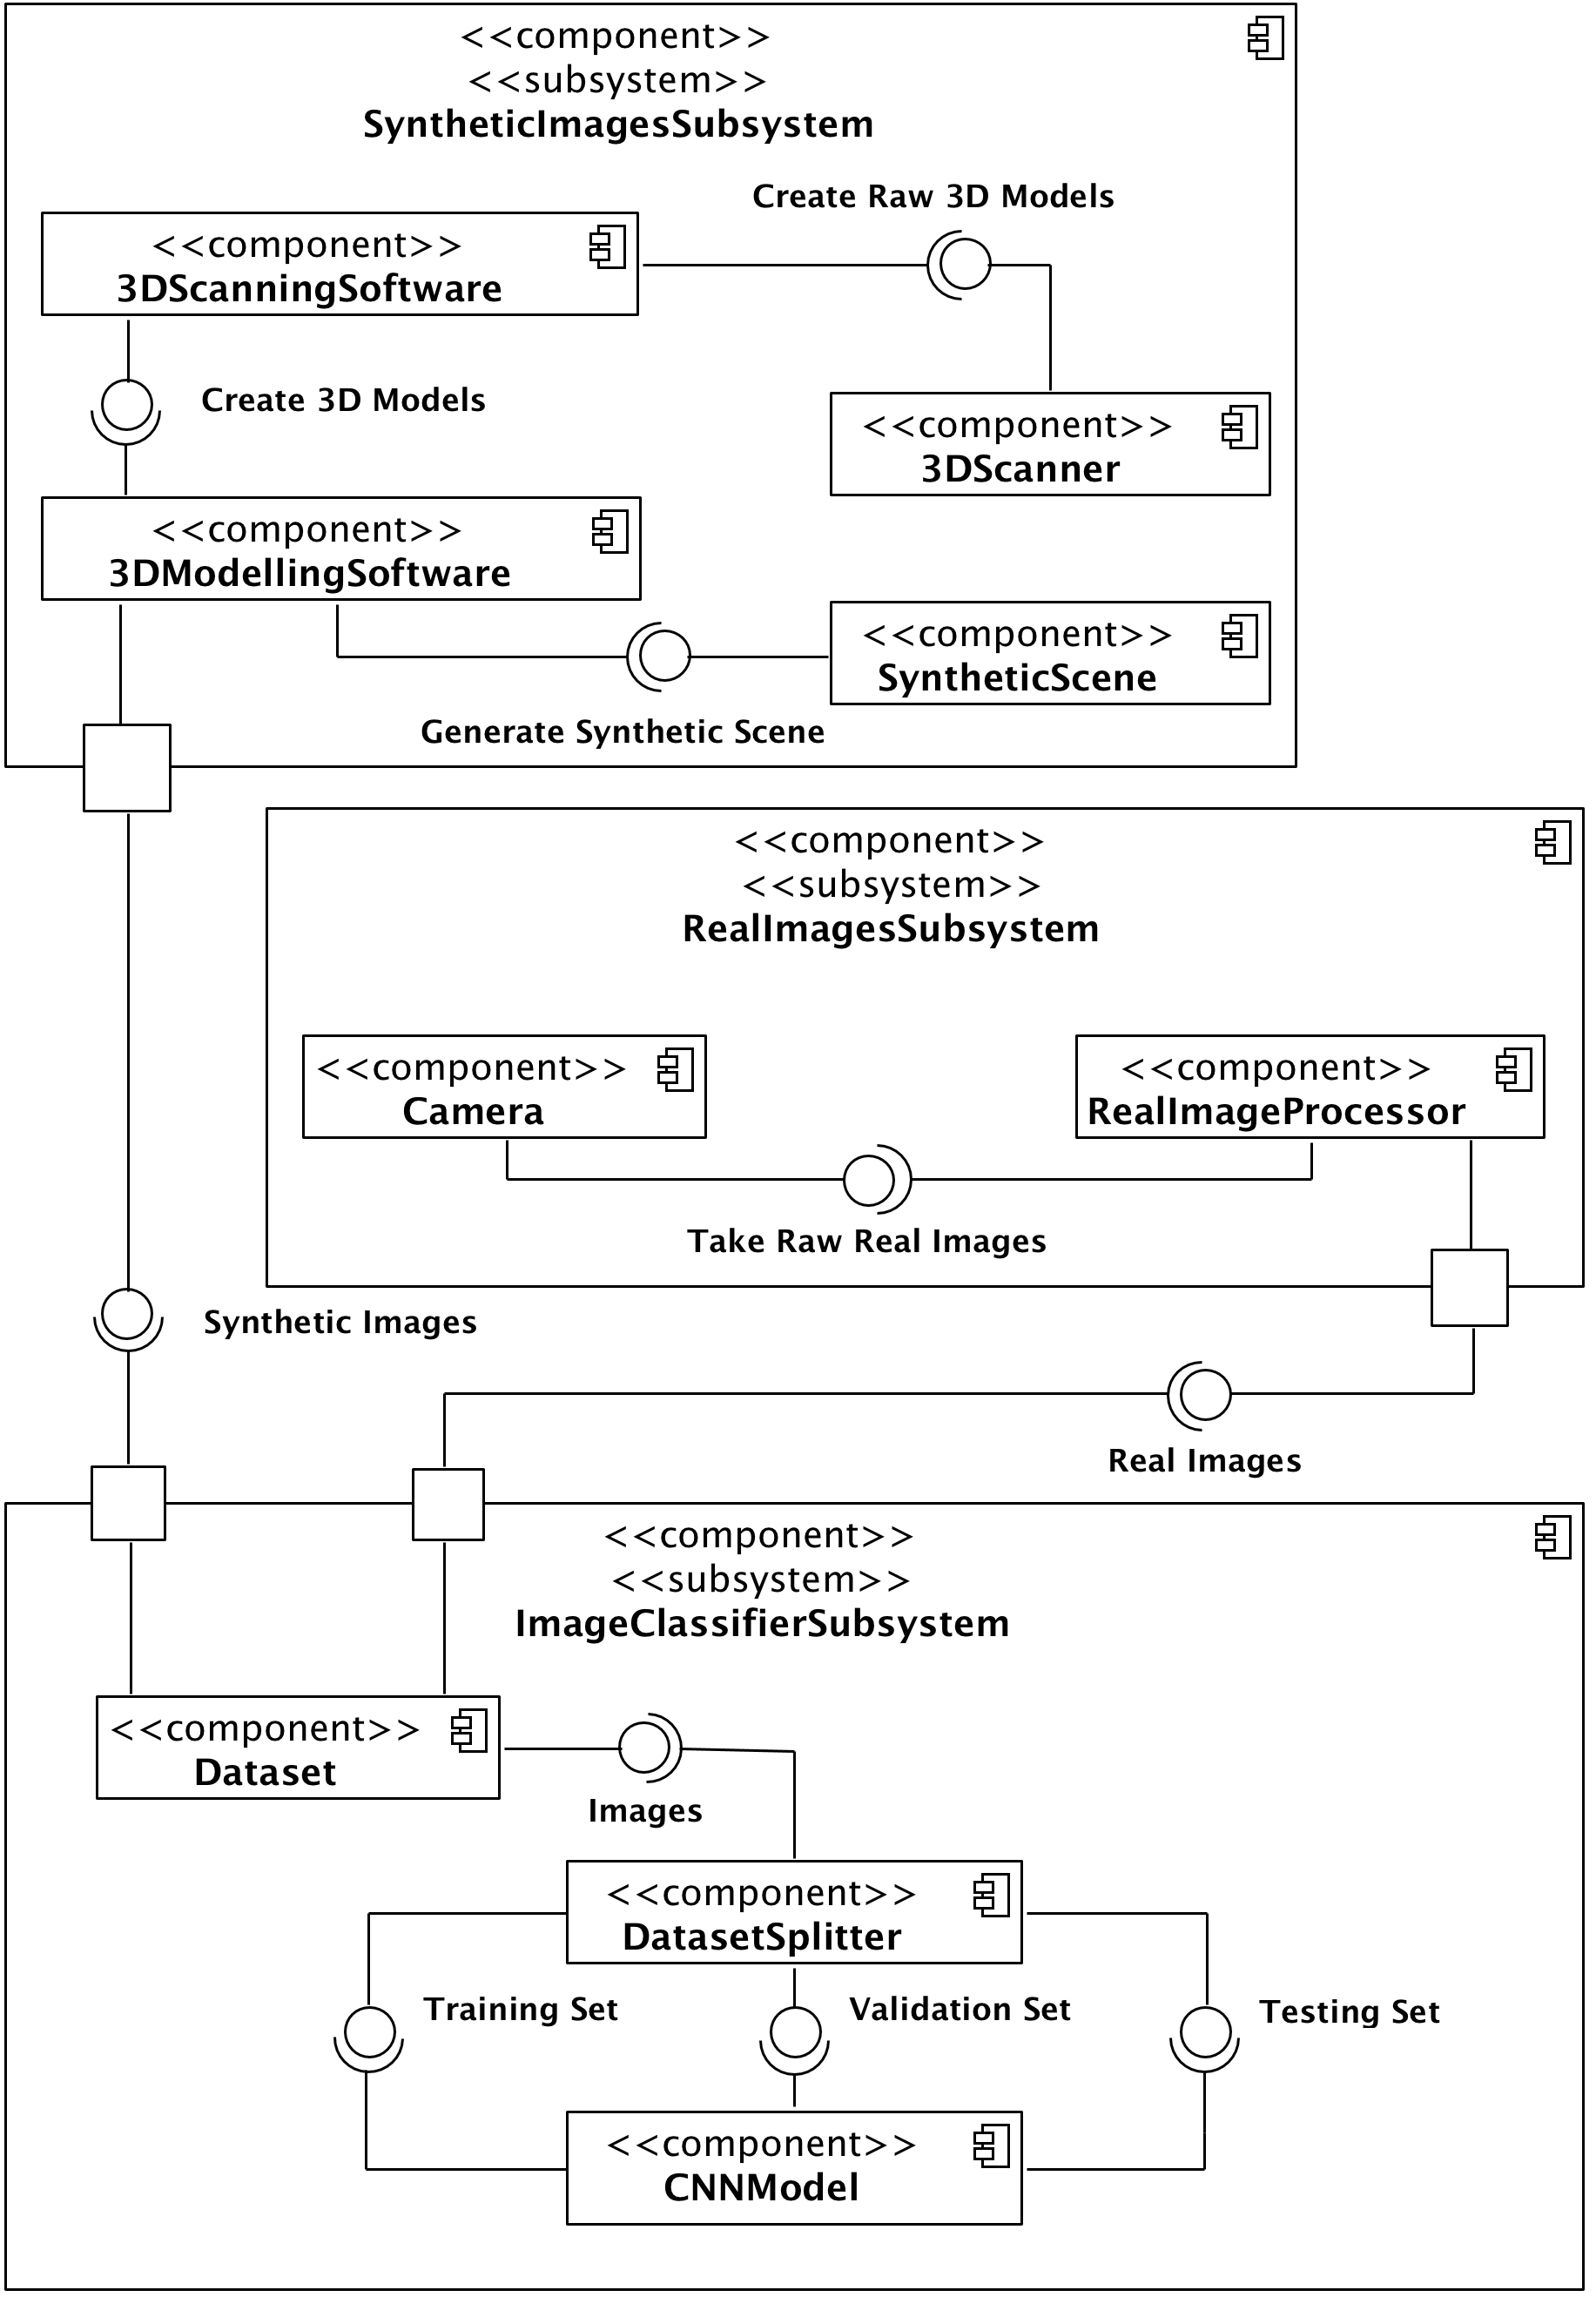
\includegraphics[width=\textwidth]{SSD}
\caption{Subsystem decomposition showing the SyntheticImageSubsystem, the RealImageSubsystem, the ImageClassifierSubsystem and the services that they provide and consume.}
\label{fig:SSD}
\end{figure}


\section{Hardware Software Mapping}\label{sec:hardware_software_mapping}

This section describes how the subsystems are mapped onto existing hardware and software components. Figure \ref{fig:DD} depicts the deployment diagram of our system. The \textbf{SyntheticImageGenerator} device is used to run 2 execution environments: the \textbf{Artec Studio}\footnote{https://www.artec3d.com/3d-software/artec-studio} 3D scanning software, and the \textbf{Rhinoceros}\footnote{https://www.rhino3d.com} 3D modeling software. Artec Studio is used to process the scans produced by the \textbf{3DScanner}\footnote{https://www.artec3d.com/portable-3d-scanners/artec-spider} device. The 3DScanner is the Artec Space Spider. The Windows version of Rhinoceros is chosen because it supports extra features that are not available on the Ubuntu or Mac versions. We use Rhinoceros to construct the SyntheticScene. Moreover, Rhinoceros hosts a \textbf{Python} execution environment. We use the Python interpreter to render synthetic images on Rhinoceros.

The \textbf{Camera} is used to capture raw images of the small parts. We use the Camera application on an iPhone 6. The \textbf{RealImageGenerator} runs a Python environment. We use the Python commands to resize the the raw images of the small parts captured by the camera. The resized real images are then ready to be fed to the image classifier.

The Dataset is stored in the file system of the \textbf{ImageClassifier} device. We use the device's Python environment to run the DatasetSplitter, the ImageClassifier, the CNNModel and the Optimizer. Furthermore, we use \textbf{Keras} \cite{chollet2015keras}, a neural networks API that provides out-of-the-box CNN implementations. The ImageClassifier device is equipped with a graphics processing unit (GPU). The GPU is used for parallel processing of the Convolutional Neural Network training algorithm. This enhancement significantly slashes down the time needed to train a CNN.

\begin{figure}[H]
\centering
  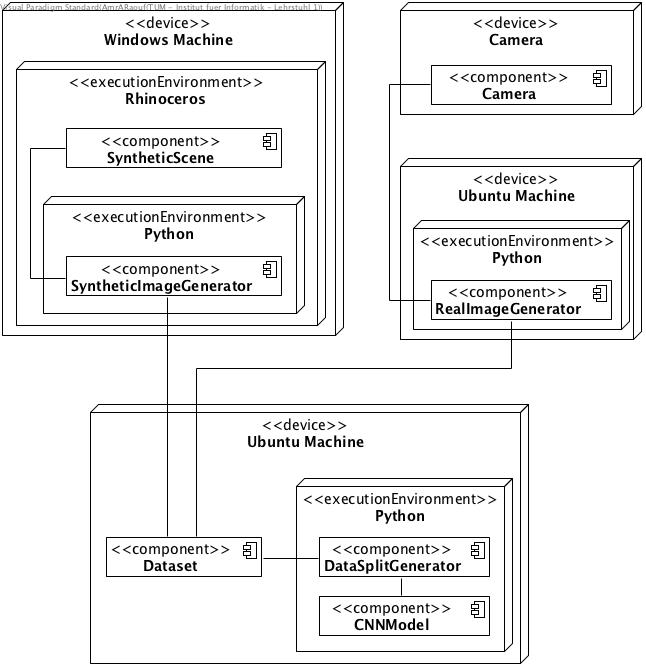
\includegraphics[width=\textwidth]{DD}
\caption{System Deployment Diagram depicting the different hardware and software components used to implement our system.}
\label{fig:DD}
\end{figure}

\section{Persistent Data Management}\label{sec:persistent_data_management}

The implementation of the ImageClassifier requires the split dataset to be organized in a certain way. The file structure of the dataset is shown in figure \ref{fig:FS}. The root folder contains 3 folders: one for training images, one for validation and one for testing. Each folder, in turn, contains one folder per class, and each of these folders are named after their respective class's label. Lastly, each class folder contains a set its own images.

\begin{figure}[H]
\centering
  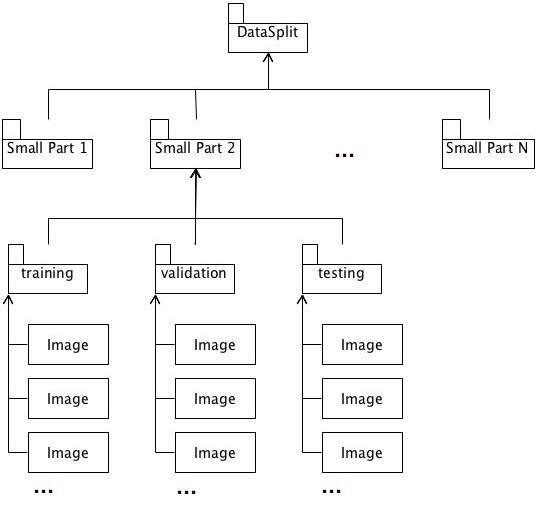
\includegraphics[width=0.8\textwidth]{FS}
\caption{Dataset file structure model displaying how the split dataset is organized before being fed as input to the image classifier. Each subfolder in the training/validation/testing directory is named after a small part label.}
\label{fig:FS}
\end{figure}

\chapter{Evaluation}

In this chapter we describe how we utilized our system to run our experiments. We provide a quantitative analysis of the data that we gathered and the comparison between the different experiment settings.

\section{Objectives}

We hypothesize that we are able to enhance the classification accuracy of our image classifier using synthetic data for training. We examine multiple ratios of synthetic to real images for training. Moreover, we run our experiments on multiple CNN architectures and fine-tune them accordingly.


\section{Methodology}

Our methodology is divided into 2 main parts: Image Collection and Training the Image Classifier. Image Collection is concerned with the real and synthetic images, and how they're collected from small mechanical parts and their corresponding 3D models. Training the Image Classifier revolves around utilizing the collected images to maximize the classification accuracy of the image classifier.

\subsection{Image Collection}

During image collection, we strive to create a synthetic dataset that has a high degree of photo-realism. Simultaniously, we want to create 3D models as fast as possible to decrease the timing of the whole workflow. To achieve this balance, we aim to create an environment that is easy to model on 3D software. We attempt to eliminate light reflections and shadows and reduce the overall complexity of the scene.

\subsubsection{Small Mechanical Parts and their corresponding 3D Models}
We first choose a small mechanical model that we wish for our image classifier to recognize. We then download the corresponding 3D model by searching the Traceparts website \cite{traceparts} for the SMP's code name.

\subsubsection{Collecting Real Images}
We place the chosen small mechanical model on a horizontal plane and place a light source underneath. We choose a plain, white, semi-transparent plane as a background to disperse the light source coming from beneath, and distribute the light evenly accross the plane. The purpose of the dispersed light is to eliminate any shadow that the small mechanical object might cast. Moreover the dispersed back light provides a lighting source without casting a direct light on the small mechanical object, which might cause glare on the SMP's reflective surface.

Next, we place a an iPhone over the plane, such that the small mechanical object is fully within the viewfield of the iPhone's camera. Our hoisting device places the iPhone 133 mm over the plane.

Afterwards, we rotate and change the position of the small mechanical part randomly, while maintaining that the SMP is fully within the viewfield of the camera. We use the iPhone's camera to take a picture of the SMP. We repeat this step until we obtain the desired number of real images.

Lastly, we resize the raw real images taken by the iPhone camera to conform with the height and width required by the image classifier.

\subsubsection{Generating Synthetic Images}
We start by creating the synthetic scene in th Rhinoceros 3D modeling software. First, we take a picture of the real horizontal plane and use it as a background for our synthetic scene. We then place a synthetic lighting source underneath the plane to mimic the lighting effect of the real environment. Next, we place the 3D model on the horizontal plane of the environment.

Next, we generate a python script that uses the Rhinoceros library to manipulate 3D objects in the Rhinoceros software. The python script is the controller for the synthetic data genertor. The synthetic data generator defines the rotation and translation ranges of the 3D model. It also specifies how many images are to be generated. For each new image, the script generates a random rotation and translation value from within the defined ranges. It then applies those transformation to the 3D model and renders a new 2D synthetic image.

\subsubsection{Dataset}


\subsection{Training the Image Classifier}


\section{Results}

\textit{Note: Summarize the most interesting results of your evaluation (without interpretation). Additional results can be put into the appendix.}

\section{Findings}

\textit{Note: Interpret the results and conclude interesting findings}

\section{Discussion}

\textit{Note: Discuss the findings in more detail and also review possible disadvantages that you found}

\section{Limitations}

\textit{Note: Describe limitations and threats to validity of your evaluation, e.g. reliability, generalizability, selection bias, researcher bias}
\chapter{Summary}

\textit{Note: This chapter includes the status of your thesis, a conclusion and an outlook about future work.}

\section{Status}

\textit{Note: Describe honestly the achieved goals (e.g. the well implemented and tested use cases) and the open goals here. if you only have achieved goals, you did something wrong in your analysis.}

\subsection{Realized Goals}

\textit{Note: Summarize the achieved goals by repeating the realized requirements or use cases stating how you realized them.}

\subsection{Open Goals}

\textit{Note: Summarize the open goals by repeating the open requirements or use cases and explaining why you were not able to achieve them. \textbf{Important:} It might be suspicious, if you do not have open goals. This usually indicates that you did not thoroughly analyze your problems.}

\section{Conclusion}

\textit{Note: Recap shortly which problem you solved in your thesis and discuss your \textbf{contributions} here.}

\section{Future Work}

\textit{Note: Tell us the next steps  (that you would do if you have more time. be creative, visionary and open-minded here.}

\appendix

\chapter{Acronyms}

\begin{acronym}
\acro{SMP}{Small Mechanical Part}
\acro{DNN}{Deep Neural Network}
\acro{CNN}{Convolutional Neural Network}
\acro{SGD}{Stochastic Gradient Descent}
\acro{GPU}{Graphical Processing Unit}
\end{acronym}


\clearpage

\listoffigures
\clearpage

\listoftables
\clearpage

\bibliography{thesis}
\bibliographystyle{alpha}

\end{document}